\documentclass{article}


% if you need to pass options to natbib, use, e.g.:
%     \PassOptionsToPackage{numbers, compress}{natbib}
% before loading neurips_2025


% ready for submission
\usepackage{neurips_2025}


% to compile a preprint version, e.g., for submission to arXiv, add add the
% [preprint] option:
%     \usepackage[preprint]{neurips_2025}


% to compile a camera-ready version, add the [final] option, e.g.:
%     \usepackage[final]{neurips_2025}


% to avoid loading the natbib package, add option nonatbib:
%    \usepackage[nonatbib]{neurips_2025}


\usepackage[utf8]{inputenc} % allow utf-8 input
\usepackage[T1]{fontenc}    % use 8-bit T1 fonts
\usepackage{hyperref}       % hyperlinks
\usepackage{url}            % simple URL typesetting
\usepackage{booktabs}       % professional-quality tables
\usepackage{amsfonts}       % blackboard math symbols
\usepackage{nicefrac}       % compact symbols for 1/2, etc.
\usepackage{microtype}      % microtypography
\usepackage{xcolor}         % colors
\usepackage{graphicx}
\usepackage{amsmath}
\usepackage{amssymb}
\usepackage{amsthm}
\usepackage{amsfonts}
\usepackage{mathtools}

\theoremstyle{plain}
\newtheorem{theorem}{Theorem}[section]
\newtheorem{proposition}[theorem]{Proposition}
\newtheorem{lemma}[theorem]{Lemma}
\newtheorem{corollary}[theorem]{Corollary}
\theoremstyle{definition}
\newtheorem{definition}[theorem]{Definition}
\newtheorem{assumption}[theorem]{Assumption}
\theoremstyle{remark}
\newtheorem{remark}[theorem]{Remark}

\bibliographystyle{unsrtnat}


\author{UNKNOWN}

\title{A Geometric Threshold for Separation Detection in Manifold Inference}

\begin{document}

\maketitle

\begin{abstract}

To analyze manifold inference, theorists typically assume continuity, while users seek separation of manifold components (e.g., MNIST). We address this component versus continuity gap directly, by asking whether a manifold consists of distinct components under different samplings. We propose a single dimensionless quantity — the ratio between the ambient distance that separates the manifold components and the largest gap in the sample cover — that tests this for a broad family of neighborhood graphs and embeddings.  For a given sampling,
when the ratio exceeds a critical threshold, manifold components remain disconnected, clustering accuracy stays high, and global distortion (measured by Gromov–Wasserstein distance) remains low; if it falls below the threshold, bridging edges appear, clusters merge, and distortion rises.  
We give upper and lower bounds for these thresholds as a function of the dimension and curvature of the data manifolds. 
This result bridges between classical (Gaussian) mixture separation principles and more topological manifold inference.

%When manifold‑learning pipelines are fed a data set that is \emph{too sparse}, distinct geometric components fuse and downstream cluster analysis fails. 
\end{abstract}

\section{Introduction}
\label{sec:introduction}



Many data–analysis pipelines start by assuming that high–dimensional observations concentrate near a low–dimensional manifold and then apply graph–based manifold learning to recover this geometry. The resulting embedding is typically clustered to discover potentially meaningful sub-populations, for example digit classes in MNIST or cell types in scRNA data. These two steps—geometry reconstruction and cluster detection—are coupled: if the sample is too sparse, neighborhood graphs acquire spurious "bridging" edges, distinct components fuse, and downstream cluster assignments fail. Practical guidelines for the sampling density required to avoid this failure are largely missing.

Under this manifold hypothesis, our data $X$ can be defined to be $X=\{x_i\}_{i=1}^n\stackrel{\text{i.i.d.}}{\sim}\nu$ with $\nu$ supported on a smooth, compact manifold $M$. From $X$ we build a neighborhood graph and an embedding map, obtaining an empirical manifold $\widehat{M}$. We therefore consider the following question: is $\widehat{M}$ the disjoint union of two or more manifolds, or has sparse sampling contributed to a falsely detected separation? 
Classical Gaussian-mixture theory provides separation guarantees in $\mathbb{R}^d$, but those guarantees neglect to consider the manifold structure of the underlying space from which our data is sampled-that is, its intrinsic geometry (e.g., curvature and reach).

We show that this connectivity decision is governed by a single dimensionless ratio: the ambient offset $\Delta$ between the underlying components divided by the fill distance $h$ of the sample. When $\Delta/h$ exceeds a curvature- and dimension-dependent threshold, no bridging edges appear in a broad class of $k$-NN and $\varepsilon$-ball graphs, and clusters remain identifiable with high probability. Below the threshold the graph connects, the manifolds fuse, and cluster labels become statistically unrecoverable, recovering the classical mixture-separation picture.

Evaluating this phenomenon raises a second challenge: one must compare "learned" manifolds that are discrete to "ground truth" manifolds that are continuous and may be sampled at different densities. To verify whether this threshold-based approach truly detects the separation of the geometry, instead of being a sampling artifact, we leveraged methods from optimal transport to define two metrics that quantify the geometric separation between manifolds at different sampling densities. Specifically, we use the Gromov–Wasserstein (GW) distance to quantify the difference between the manifold approximations at each stage of the manifold inference pipeline. We show our metrics converge as the sampling density increases, and that the Gromov–Wasserstein distortion between $\widehat{M}$ and a densely sampled reference stays low. This allows us to verify that the clusters remain distinct, and that the manifold inference pipeline is able to recover the geometry of the underlying manifold.

\begin{figure}[t]
    \centering
    \includegraphics[width=0.8\linewidth]{figures/Fig1V3.jpg}
    \caption{A topological view of manifold components separation. (top) Suppose data are drawn from a non-simple manifold consisting of two separate geometries. Fill distance ($h_1, h_2$) provides a measure of spread (solid lines), is dependent on sampling, and may exceed the separation between components ($\Delta$). Their ratio exhibits a threshold criterion in Gromov-Wasserstein distance. (bottom) k-nearest-neighbor graphs vary as a function of sampling density around the threshold.
    }
    \label{fig:manifold_sampling}
\end{figure}

In summary, we make the following contributions:
\begin{enumerate}
    \item \textbf{Geometric criterion for cluster preservation.} We introduce the offset–fill-distance ratio and prove upper and lower thresholds that predict when clusters remain distinct. Theorem~\ref{thm:knn-threshold} and Figure~\ref{fig:dim-aggregate} give theoretical and empirical support.
    \item \textbf{Metric-based evaluation of manifold embeddings.} We employ Gromov--Wasserstein distance to compare learned manifold representations against densely sampled reference manifolds, yielding a measure of global geometric similarity for practical evaluation.
\end{enumerate}

Together these results offer an interpretable test for deciding when manifold-learning pipelines can reliably separate meaningful components in high-dimensional data. 


\section{Background}
\label{sec:related-work}
Below, we provide a brief review of concepts that inform our work, specifically manifold inference, classical cluster separation via mixture models and the motivation of our work from the perspective of differential geometry.

\paragraph{Manifold Inference.}
Manifold inference algorithms aim to map high-dimensional data onto a lower-dimensional representation while preserving local geometric properties. Classical methods such as Isomap \cite{tenenbaumGlobalGeometricFramework2000}, Laplacian Eigenmaps \cite{belkinLaplacianEigenmapsDimensionality2003}, and Locally Linear Embedding \cite{roweisNonlinearDimensionalityReduction2000} rely on neighborhood-graph approximations and shortest-path distances. More recent algorithms like t-SNE \cite{maaten2008tsne} and UMAP \cite{mcinnesUMAPUniformManifold2020} optimize probabilistic or topological objectives to capture both local and some global data structure. Most methods utilize a two-step approach, where the first involves using a similarity kernel to define a weighted "data graph", and thereafter using a spectral or optimization-based approach to construct a visualizable embedding.  \cite{meilaManifoldLearningWhat2023}. 

\paragraph{Gaussian Mixtures.}
The problem of developing algorithms to learn the distributions of data sampled from \emph{Gaussian Mixture Models (GMMs)} has been well-studied over the past two decades. Classic results show that statistical approaches can solve this problem when sufficient separability and sampling of data points exist, where the bounds are functions of the distance between centers of Gaussians, the variance of the distributions and the dimensionality of the space. \citet{aroraLearningMixturesSeparated2005, vempalaSpectralAlgorithmLearning2004} Spectral clustering approaches also leverage similarity graphs and eigen-decompositions to detect partitions in data \citet{luxburgTutorialSpectralClustering2007}, but these face the same obstacles as manifold inference algorithms: they rely on the choice of similarity kernel.

\begin{figure}[t]
    \centering
    \includegraphics[width=0.8\linewidth]{figures/Fig2V2.jpg}
    \caption{Highlighting the limitations of Mixture Models for determining separations in manifold data. The geometry of the data does not admit a natural notion of mean and variance, instead the Gaussian assumption in (a) leads to the curvature of the manifolds being overlooked and the overlap being overestimated. This artifact is remedied in (b) by considering the ambient offset, thus respecting the geometry-specifically the reaches-of the manifolds to ensure the fill distance remains controlled preventing the likelihood of overlap between the two manifolds.}
    \label{fig:manifold_convergence}
\end{figure}

\paragraph{Relationship to Reach.}
In classical differential geometry, the \emph{reach} \(\tau_M\) of a smooth, boundary‑free manifold \(M\subset\mathbb{R}^D\) quantifies the largest radius for which every point in the tubular neighborhood of \(M\) admits a unique projection back onto \(M\).  Equivalently, \(\tau_M\) is the infimum distance from \(M\) to its \emph{medial axis}, the set of points having more than one nearest neighbor on \(M\) \cite{feffermanReconstructionInterpolationManifolds2020}.  Reach thus captures both local curvature—since \(\tau_M\) is bounded above by the reciprocal of the largest principal curvature—and global bottlenecks—since narrow “necks” between distant parts of \(M\) force \(\tau_M\) to shrink.  In practice, modern estimators can recover \(\tau_M\) from point samples: for instance, Aamari et al.\ provide minimax‑optimal rates \cite{aamari2019estimating}, and Boissonnat and Wintraecken analyze how reach behaves under unions manifolds \cite{boissonnat2023reach}.

Our offset–fill‑distance ratio \(\Delta/h\) can be viewed as a relaxation of reach for the case of distinct components.  Here, \(\Delta\) is the minimal ambient separation between two disjoint manifold pieces, playing the role of twice the bottleneck radius in the medial‑axis formulation, while \(h\) is the fill distance of the sample, measuring the worst‑case sampling gap. Demanding \(\Delta/h\) exceed a critical constant mirrors the requirement that sampling density lie below the reach, thereby avoiding spurious graph connections. As reach closely relates to curvature, one should note that an estimate of curvature is required for our approach as well. Existing work considers the problem of estimating curvature from intrinsic point‑cloud methods \cite{hickok2023intrinsic}, as well as methods to define the closeness of different manifolds using a notion of flat distance \cite{sormani2011intrinsic}. However, a key quality of our work is that we are focused on the (reach of the) free space between manifold components rather than within a pure manifold, thus connecting the geometry to our algorithmic task.



% , which our approach attempts to do from a more classical separation-based approach. 


% To assess embedding quality beyond simple pairwise distortion metrics, many have increasingly begun to consider to \emph{optimal transport} methods. In particular, \emph{Gromov--Wasserstein (GW)} distance compares pairs of metric measure spaces by finding an optimal correspondence between their points \citet{memoliGromovWassersteinDistances2011}. GW is well suited to manifold inference problems, as it captures intrinsic geometric discrepancies between two point clouds (e.g., a learned manifold vs.\ a more densely sampled reference) without assuming they lie in the same ambient space.

\section{Geometric Cluster-Separation Criterion}
\label{sec:geom-criterion}

We now introduce our main theoretical framework for understanding cluster separability on manifolds. Drawing parallels to Gaussian Mixture Models, we regard \emph{offset} as the analog of inter-cluster distance and \emph{fill distance} as a proxy for “variance” or dispersion within each manifold component.

\subsection{Defining Offset and Fill Distance for Manifolds}
\label{sec:offset-fill-definition}

Suppose our data lie on the union
$$
\mathcal{M} \;=\; \mathcal{M}_1 \cup \cdots \cup \mathcal{M}_K,
$$
where each $\mathcal{M}_k$ is a connected manifold component in $\mathbb{R}^D$. Let
$$
\Delta \;=\; 
\min_{k\neq \ell}\,\Bigl\{\rho_{\mathbb{R}^D}(x,y)\colon x\in\mathcal{M}_k,\,y\in\mathcal{M}_\ell\Bigr\}
$$
be the minimal ambient distance between distinct components (i.e., the \emph{offset}). In parallel, define the fill distance for $\mathcal{M}$ sampled approximation as follows.

\begin{definition}[Fill Distance] \label{sec:prelim-filldist}
Let $R = \{r_i\}_{i=1}^n \subset \mathcal{M}$ be a finite point set. The \emph{fill distance} is
$$
h_{R,\mathcal{M}} \;=\; \sup_{x \in \mathcal{M}}\, \min_{1 \leq i \leq n} \|x - r_i\|.
$$
We say $R$ is \emph{quasi-uniform} if $h_{R,\mathcal{M}}$ and the minimum pairwise distance among $r_i,r_j$ differ only by a constant factor. A small fill distance indicates that $R$ forms a dense covering of $\mathcal{M}$.
\end{definition}

\begin{remark}
    In analogy to the sampling density criterion and variance in Gaussian Mixture Models, we treat fill distance $h_{R,\mathcal{M}}$ as a measure of \emph{sampling dispersion}. A smaller $h_{R,\mathcal{M}}$ translates to higher sampling density, which is often necessary for manifold learning algorithms to reliably approximate geodesic distances and local neighborhoods.
\end{remark}

We denote $h_{R,\mathcal{M}}$ as $h$ for convenience and then form the following ratio
$$
R \;=\; \frac{\Delta}{h},
$$
% Empirically, if $R$ exceeds an application-dependent threshold $R_0$, the manifold clusters remain distinct; if $R<R_0$, the data graph or embedding procedure often merges clusters or distorts their geometry. The intuition for this is that at the boundary threshold, manifold inference algorithms can often incorrectly form spurious connections between distinct features due to how the heuristics chosen to form this data graph often rely on the density of the samples. Fill distance provides a geometric notion of density which is designed to make this threshold tight. See Figure~\ref{fig:manifold_convergence} for further intuition. Particularly, as we increase fill distance the density decreases, making the role of the offset more important in preventing spurious connections and vice versa. This is particularly important as many kernel estimation algorithms rely on density-based criteria to define notions of pairwise similarity \cite{dyballaIANIteratedAdaptive2023a}. We now offer the following technical result justifying the existence of this threshold: 

We now establish a sharp threshold phenomenon for the connectivity of a \(k\)-nearest neighbor ( \(k\)-NN) graph constructed on points sampled from two disjoint, compact \(d\)-dimensional Riemannian manifolds. That is, we show how the connectivity of a k-NN graph on points sampled from two separate manifolds undergoes a sharp phase transition: if the distance between the manifolds (relative to the scale at which the points cover each manifold) is too large, no edge will bridge them, but if it is small enough, a bridging edge is likely to appear. In other words, under the assumption that clusters are separate iff they are sampled from two different manifolds, this theorem quantifies how sampling density (as measured by the fill distance) and the intrinsic separation of the clusters determines whether the clusters remain disconnected or connected in the graph.


\begin{theorem}[Threshold for Manifold Separation in the k-NN Graph]
\label{thm:knn-threshold}

Let $\mathcal{M}_1$ and $\mathcal{M}_2\subset\mathbb{R}^D$ be two disjoint, compact, $d$-dimensional manifolds with uniform sampling. Let $\Delta>0$ be their ambient offset, and let $h_{\max}$ is the maximum fill distance when sampling $n_1$ points in $\mathcal{M}_1$ and $n_2$ points in $\mathcal{M}_2$. Construct the $k$-NN graph on all $n=n_1+n_2$ points with $k = \log(\frac{n}{\delta}) + d$. We then have under these assumptions that there exist constants $\widetilde{C},\widehat{C}>0$ (depending on $d$, the manifold geometries, and $k$) such that with high probability the following holds:
\begin{enumerate}
    \item If 
    \[
    \frac{\Delta}{h_{\max}} \;>\; \widehat{C},
    \]
    then no edges connect $\mathcal{M}_1$ and $\mathcal{M}_2$ in the $k$-NN graph.
    \item If 
    \[
    \frac{\Delta}{h_{\max}} \;<\; \widetilde{C},
    \]
    then there is a high probability that the $k$-NN graph contains an edge joining a point in $\mathcal{M}_1$ to $\mathcal{M}_2$.
\end{enumerate}
In other words, the ratio $\Delta/h_{\max}$ determines whether the $k$-NN graph is disconnected (one component per manifold) or exhibits at least one bridging edge. Moreover, under the local volume conditions the constants $\widetilde{C}$ and $\widehat{C}$ can be explicitly taken as
\[
\widetilde{C} = \frac{1-\varepsilon}{2}\Bigl(\frac{c_1}{c_2}\Bigr)^{1/d},\quad
\widehat{C} = \frac{1+\varepsilon}{2}
\]
where $c_1$ and $c_2$ correspond to the maximum sectional curvatures of $\mathcal{M}_1$ and $\mathcal{M}_2$ respectively. These bounds on the estimates of $\widetilde{C}$ and $\widehat{C}$ hold with probability $1 - \delta$.
\end{theorem}

\paragraph{Proof Sketch.} We begin by establishing a high-probability bound on the fill distance $h$ via a standard covering argument using epsilon balls over the entire manifold. Our main bounded local volume assumption arises from the seminal work of \citet{niyogiFindingHomologySubmanifolds2008a}.
Applying standard Chernoff bounds shows that the $k$th-nearest neighbor distance $D_k(x)$ concentrates around a scale proportional to $h$, so that for all $x\in\mathcal{M}$ we have $\widetilde{C}\,h\le D_k(x)\le \widehat{C}\,h$. This correspondence yields two cases: if $\Delta> \widehat{C}\,h_{\max}$ then all $k$-NN edges remain within each manifold (ensuring disconnection), whereas if $\Delta< \widetilde{C}\,h_{\max}$, local neighborhoods on the two manifolds overlap, and a bridging edge exists with high probability. Corollaries then follow, providing analogous bounds for RBF kernel bridging weights, and the same arguments extend to nonuniform measures satisfying similar two-sided volume conditions. We offer the complete proof of this result in the Appendix~\ref{app:knn-threshold-proof}. 

% \begin{figure}[t]
%     \centering
%     \includegraphics[trim=0pt 100pt 0pt 100pt, clip, width=0.8\linewidth]{figures/Fig4V1.png}
%     \caption{This figure highlights the intuition behind fill distance $h$ and offset $\Delta$. At the boundary threshold, manifold inference algorithms can often incorrectly form spurious connections between distinct features due to the lack of density in the points from the intrinsic geometry they are attempting to learn.  }
%     \label{fig:fill_dist_intuition}
% \end{figure}

\section{Manifold Inference Metrics}

\paragraph{Motivation.}
Manifold learning can be viewed through a statistical lens in which data points are drawn from a probability distribution supported on a low-dimensional manifold embedded in a high-dimensional ambient space. As the sample density increases, one expects the discrete graph constructed from data points to approximate the manifold’s geometry and topology with greater accuracy. Classical results show, for example, that graph Laplacians converge to the continuous Laplace-Beltrami operator of the manifold when sampling is uniform and certain smoothness conditions are met~\citet{belkinConvergenceLaplacianEigenmaps2007, trillosErrorEstimatesSpectral2018}.

More recent work extends these findings beyond uniform sampling. Particularly, \citet{soberApproximatingRiemannianMetric2020} and \citet{trossetRehabilitatingIsomapEuclidean2021} analyze how the shortest-path metrics of algorithms like Isomap converge to the manifold’s geodesic distances as sampling density improves, even under mild deviations from uniformity. Such convergence results imply that, in the limit of abundant data, the discrete metric measure space induced by a sufficiently dense sample can recover a large portion of the manifold’s intrinsic distances and global structure (i.e. organization of clusters).

If a reference manifold approximation is constructed from a large, carefully sampled dataset, we can treat it as a practical stand-in for the unknown ground-truth manifold. As discrete approximations become more faithful, they should converge in a suitable metric to this reference. In the case of shortest-path metrics, this implies that the sample graph approximation of the true geodesics. Path distances offer a further benefit in that under mild assumptions on the curvature and compactness of the underlying manifold, they define the manifold up to homeomorphism. \cite{Nik83}

% While manifold inference often aims at dimensionality reduction for visualization or analysis, quantifying the embedding’s accuracy becomes difficult particularity when the data is sampled insufficently. Many algorithms preserve local neighborhoods or spectral properties, but these objectives do not necessarily guarantee faithful retention of global structures, such as the number of distinct clusters or overall topology.

\paragraph{Gromov--Wasserstein (GW) Metric.}
To define metrics with aforementioned convergence properties, our approach relies upon using Gromov--Wasserstein (GW) distance \citet{memoliGromovWassersteinDistances2011}. Unlike standard reconstruction error metrics, GW compares two metric measure spaces holistically by finding an optimal matching between their points. In practical terms, this allows us to compare a low-dimensional embedding of the manifold to a denser or more uniform reference manifold, validating whether crucial geometric features (e.g., distinct clusters) are preserved.

Beyond purely geometric considerations, GW distances can be incorporated into evaluating the cluster structure of the final embeddings. Prior work has shown that through marginal changes to classical linkage-based hierarchical clustering, we can define hierarchical clustering which generate dendrograms with finite sample convergence guarantees as the sample density increases. ~\citet{chaudhuriConsistentProceduresCluster2014} Further work has shown that treating dendrograms yielded through linkage-based clustering algorithms induce ultrametric spaces with the property that the GW distance on the ultrametric spaces are stable in the Gromov-Hausdorff sense \cite{carlssonCharacterizationStabilityConvergence}. Thus, justifying the use of GW distance on the dendrograms to assess the distortion of the embedded data.


\subsection{Theoretical Results on Gromov--Wasserstein Convergence}
\label{sec:theory-GW-convergence}

We first recall the following definition.
\begin{definition}[Gromov--Wasserstein Distance]\label{def:GW-Dist}
Let $(X,d_X,\mu_X)$ and $(Y,d_Y,\mu_Y)$ be two compact metric measure spaces. The \emph{p-Gromov--Wasserstein distance} ($p\ge1$) is defined as
$$
% GW_p\bigl((X,d_X,\mu_X),(Y,d_Y,\mu_Y)\bigr)
% \;=\;
\inf_{\pi \in \Gamma(\mu_X,\mu_Y)} \!\Bigl(\iint_{X\times X\times Y\times Y}
\bigl|\,d_X(x,x') - d_Y(y,y')\bigr|^p
\,d\pi(x,y)\,d\pi(x',y')\Bigr)^{\!1/p}
$$
where $\Gamma(\mu_X,\mu_Y)$ is the set of all couplings of $\mu_X$ and $\mu_Y$.
\end{definition}

Prior work has shown that if certain knowledge of the reach, curvature, etc of the manifold is known apriori, manifold learning algorithms can approximate $(\mathcal{M},\rho_{\mathcal{M}})$ by sampling a finite set $R$ with fill distance $h$, producing $(M_h, \rho_{M_h})$, with the property that:
$$
\rho_{M_h}(P_h(x), P_h(y)) \;=\; \bigl[1 + O(h^{\,k-1})\bigr] \,\rho_{\mathcal{M}}(x,y),
$$
for all $x,y\in \mathcal{M}$, where $P_h:\mathcal{M}\to M_h$ is a homeomorphism and $k\ge2$ depends on the manifold’s smoothness~\citet{soberApproximatingRiemannianMetric2020}. 

This result on the bounded distortion of the shortest-path metric allows us to show the following.
\begin{theorem}
If $\mu$ is a probability measure on $\mathcal{M}$, under assumptions outlined in \ref{assump:manifold-inference} on $\mathcal{M}$ and the inference algorithm, then the natural pushforward via $P_h$ yields $\mu_h$ on $M_h$, giving
$$
GW\Bigl((\mathcal{M},\rho_{\mathcal{M}},\mu), (M_h,\rho_{M_h},\mu_h)\Bigr) 
\;\le\; C\,h^{k-1}.
$$
\end{theorem}

Hence, finer sampling (smaller $h$) leads to more faithful reconstructions in $GW$ distance. We defer the technical details to Appendix~\ref{thm:gw-main-app}, but note these results ensure the rate of convergence of this metric is controlled, justifying the use of the discrete manifold approximation when comparing data that is sparse relative to the complexity of the manifold. The proof of the result follows directly from applying the result from \citet{soberApproximatingRiemannianMetric2020} to Definition~\ref{def:GW-Dist} and leveraging basic properties of metric spaces. We also show a similar result in Appendix~\ref{thm:SL-stability} for the use of optimal transport on linkage-based dendrograms. We show a weaker convergence argument-that the GW distance goes to zero between the ultrametric spaces derived from dendrograms-by leveraging standard properties of GW and the results from \citet{chaudhuriConsistentProceduresCluster2014}. We offer this result to justify the use of this second GW metric to compare embeddings with varying sample sizes.


\section{Empirical Evidence}
\label{sec:Empirical Evidence}

\subsection{Experimental Setup}
\label{sec:methodology-setup}

We generated synthetic datasets in $\mathbb{R}^D$ by uniting multiple geometric shapes (spheres, ellipsoids, hyperboloids and tori), each sampled at a specified density. An \emph{offset} parameter determined how far these shapes were placed from one another, controlling the inter-cluster distance. From each full dataset, we extracted smaller subsamples at different fractions (e.g., 100\%, 50\%, 10\%), using uniform, biased and noisy sampling procedures. Subsamples allowed us to examine the role of fill distance: the sparser the sampling, the larger the fill distance. We computed fill distance after each subsampling using the k-nearest neighbor approximation from Lemma~\ref{lem:nn-concentration}-averaging the distance of every point to its k-th nearest neighbor-to quantify sampling resolution relative to offset (Section~\ref{sec:geom-criterion}). In all cases, the full datasets served as approximate “ground truth,” providing ground truth labels for clustering assignments and enabling us to measure global distortions caused by insufficient coverage. 

% Although our main experiments focused on \emph{uniform sampling}, our pipeline also accommodated non-uniform (biased) sampling based on potential functions (Appendix~\ref{app:sampling-details}). We recorded pointwise labels—either identifying the shape in a union-of-shapes dataset or the component in a Gaussian mixture—allowing us to measure clustering accuracy when a partition of the manifold was known a priori.

\begin{figure}[t]
\centering
\includegraphics[width=0.8\linewidth]{figures/Fig3V3.jpg}
\caption{Conceptual overview of the experimental pipeline, from dataset construction through final evaluations. For each configuration of manifolds with centers separated on the vertices of a $\Delta$-scaled maximal dimensional unit simplex, (1a) the dense "reference" approximation pipeline and (1b,1c) represents the sparse, noisy samples. (2) depicts the graph induced by the convex hull for (2a) and the variable kernel method for (2b,2c). The GW Path metric (i) compares (2a) and (2b,2c). (3a) depicts the spectral clustering embedding of the graph from (2a) and similarly for (3b, 3c) the variable embedding of (2b,2c) data. (3a), (3b) and (3c) admit hierarchical clustering graphs (4a), (4b) and (4c) which are compared using the ultrametric GW distance (ii).}
\label{fig:pipeline-experiment}
\end{figure}

% \paragraph{Adjacency Kernel Constructions}
% \label{sec:methodology-kernels} 
After subsampling, we constructed a graph whose edges approximate manifold distances. Each adjacency matrix was built using one of the following kernels or graph-based schemes:
\textit{Gaussian (RBF) Kernel},
\textit{$k$-NN Graph with Pruning}
where pruning removed spurious edges using heuristics including:
MST-based pruning \cite{MSTShaoChaoZhao2007}, 
distance-based pruning, 
density-based pruning and bisection-based pruning \cite{TianLiZhangBisection}. 
We considered additional adjacency definitions, including a parameter-free volume-based kernel (IAN) as well as the adjacency derived from t-SNE perplexities. \cite{dyballaIANIteratedAdaptive2023a} Each adjacency matrix was symmetrized, and all disconnected components were handled by assigning large pairwise distances between them. Finally, we computed the shortest-path distance matrix on the resulting graph, approximating geodesics.

% \paragraph{Manifold Embedding Algorithms}
% \label{sec:methodology-embedding} 
We embedded the shortest-path distance matrices (or their equivalent affinity matrices) into a lower-dimensional space (usually 2D), comparing a variety of manifold learning algorithms: \emph{Isomap} \citet{tenenbaumGlobalGeometricFramework2000, trossetRehabilitatingIsomapEuclidean2021}.  
\emph{Locally Linear Embedding (LLE)} \citet{roweisNonlinearDimensionalityReduction2000}.  
\emph{Laplacian Eigenmaps}, \emph{Diffusion Maps} \citet{belkinLaplacianEigenmapsDimensionality2003, coifmanDiffusionMaps2006}. 
\emph{t-SNE} and \emph{UMAP} \citet{maaten2008tsne, mcinnesUMAPUniformManifold2020}. All methods were used in their standard library implementations with a standard range of fixed hyperparameters (see Appendix~\ref{app:params}) to ensure consistency and mimic practical usage.

\paragraph{Evaluation Metrics.}
\label{sec:methodology-metrics} 
% \paragraph{Global Distortion via Gromov--Wasserstein (GW).}
Let $D_{\text{full}}$ be the distance matrix for the entire dataset (i.e., a high-density reference) and $D_{\text{sub}}$ the distance matrix for a subsampled graph. We treated each set of points as a metric measure space with uniform distributions. The \emph{2-Gromov--Wasserstein distance} was computed using the sinkhorn optimization procedure to compute the cost of optimal transport plan and quantify how well $D_{\text{sub}}$ can be optimally matched to $D_{\text{full}}$. Larger GW cost indicated greater distortion.

% \paragraph{Clustering and Hierarchical Consistency.}
Since each synthetic dataset had a known partition, we used \emph{Adjusted Rand Index (ARI)} to measure how well $k$-means clustering recovered these labels for known $k$. $\mathrm{ARI}=1.0$ signifies perfect agreement, whereas $0$ indicates random clustering. We also extracted \emph{stable linkage-based hierarchical clustering} from both the subsampled data and the full dataset. Using the ultrametric spaces induced by these dendrograms, we then approximated their discrepancy using the Gromov-Wasserstein distance with uniform measure on both spaces with the same sinkhorn-based optimization procedure for GW computation (Appendix~\ref{app:ultrametric-details}). This revealed whether the structure in the cluster embeddings, such as the separation of connected components, remained intact across sampling densities.

\paragraph{Real Data.} To validate our theory on real data, we employed the MNIST~\cite{MNIST} dataset and single-cell RNA data, specifically 3k PBMCs from~\cite{pbmc3k_2016}. Since we cannot control the offset, we instead employed the natural test our ratio-based threshold exhibits for pairs of clusters, according to Theorem~\ref{thm:knn-threshold}. We do this by computing hypothesized clusters using kmeans and spectral clustering for a specific $k$, and for every pair of proposed clusters we compute the ratio. Using the lower confidence bound of $0.5$ from Theorem~\ref{thm:knn-threshold}, we plot the percentage of pairs from all possible pairs of clusters above $0.5$. We conducted this procedure on sampled data points from these datasets. For this threshold to function, we expect the percentage of ratio crossing pairs will increase significantly when we reach the expected number of clusters (i.e. 10 for MNIST and 5 for scRNA).

\section{Results}
\label{sec:results}

\paragraph{Synthetic Experiments.}
We first examine representative synthetic scenarios, each comprising a union of manifolds of varying geometries and topologies. Specifically, we considered a sphere, torus, ellipsoid and hyperboloid, of dimensions varying from 2 to 25, with varying offsets, sampled uniformly, with bias and with noise at different sampling densities. Figure~\ref{fig:dim-aggregate} illustrates summaries of the plots for the uniform sampling case for data at dimension 5, 15 and 25. Each of three line plots plot the following quantities respectively: (1) ARI, quantifying cluster accuracy relative to true labels, (2) Graph GW, measuring the global geodesic distortion, and (3) Tree GW, quantifying the distortion in the embedding. As depicted in the figure, each plot at each dimension depicts the threshold being present with sudden changes for specific ratio values. That is, the ARI jumping and remaining high at roughly the same threshold that the Graph GW and Tree GW metric distortion decreases substantially. It did seem slightly less noticeable in the Graph GW distance for higher dimensions, which is likely an artifact of the concentration of measure phenomenon-also known as the curse of dimensionality-that occurs with distances in higher dimensions. We further note that for biased and noisy data, we observed this same behavior of the threshold existing but in a less pronounced way for the Graph GW metric, further confirming the difficulties of quantifying this threshold in settings that are not sampled uniformly from low-dimensional, smooth compact manifolds.

\paragraph{Real Data Experiments}
We consider the optimal cluster search using kmeans and spectral clustering for MNIST and scRNA data. As depicted in Figure~\ref{fig:MNIST}, we see that for both MNIST and scRNA, there is a significant uptick in the percentage of pairwise proposed clusters whose ratio exceeds the threshold precisely at the point where we expect the true number of clusters to occur. We highlight that while we would hope this percentage to be higher, there are known limitations with kmeans and spectral clustering in their ability to identify the correct cluster regions of MNIST completely, so the existence of this uptick in spite of this is promising. Furthermore, visually the TSNE and UMAP plots for both MNIST and scRNA do not offer clear visual cluster distinctions, so this further confirms the usefulness of this threshold criterion in determining true separation of clusters in high-dimensional data. We lastly note that in the scRNA plot for percentage of pairwise thresholds over number of clusters, the substantial increase after the first $5$ clusters is likely due to the use of the lower bound threshold from the theory. Given that this lower bound omits curvature, which is necessary for a higher confidence bound on this threshold, this is likely the reason for the substantial increase after the initial uptick.


\begin{figure}[t]
\centering
\includegraphics[width=0.8\linewidth]{figures/Fig4VNovel.jpg}
\caption{A summary of our synthetic experiments. The three rows depicted each contain the results of ARI, Graph GW and Tree GW for dimensions 5 (top), 15 (middle) and 25 (bottom), all plotted against the ratio (offset/fill distance). The left column (a) depicts TSNE plots of the 5 dimensional data for increasing offset, and the right column (b) depicts TSNE plots for 15 dimensional data, here with increasing fill distance as one proceeds downwards. The main three row plots for the different dimensional synthetic data all depict the presence of a threshold where cluster detectability suddenly increases and geometric distortion in the data graph and embedding decrease.}
\label{fig:dim-aggregate}
\end{figure}

\begin{figure}[t]
\centering
\includegraphics[width=0.8\linewidth]{figures/Fig5VFinal.jpg}
\caption{Results of our search for optimal clusters using the theoretical threshold estimate of $0.5$ for MNIST (a) and for the scRNA data (b). For (a), we notice that as MNIST is known to have 10 clusters, our analysis shows a significant rise at this point specifically, and a similar phenomenon occurs for the scRNA data which is known to have an identifiable 5 clusters present. The GW plots for MNIST in (a) show a threshold existing when the inverse fill distance of samples reaches a certain point, and the three UMAP and TSNE plots for MNIST and scRNA depict the lack of clear visual separation in the clusters that were still identifiable using the threshold plotting approach.}
\label{fig:MNIST}
\end{figure}


\section{Discussion}
\label{sec:discussion}

\paragraph{Limitations.}
While the results of this paper offer compelling evidence on the existence and usefulness of this threshold, our theoretical results do make stricter assumptions on the underlying manifolds themselves. That is, we require each component to be a smooth, positive-reach manifold and we treat sectional curvature as if it were known, yet as real data often contain outliers, boundaries, or noise, this can lead to regions where sectional curvature may not even be defined. Addressing this remains an open challenge. 
Further, graph-based estimators of curvature such as Ollivier–Ricci can have high variance, leading to the constants \(\widetilde{C},\widehat{C}\) in Theorem \ref{thm:knn-threshold} requiring greater confidence intervals and reducing the precision of the threshold test in practice. \citet{saidiRecoveringManifoldStructure2024}

\paragraph{Future directions.}
In spite of these limitations, three extensions of this work follow naturally. First, as the use of this threshold currently relies on existing hypothesis clusters to be predefined, one potential extension is that of creating a density-based clustering algorithm that utilizes the empirical ratio \(\widehat{\mathcal{R}}=\widehat{\Delta}/h\) as a greedy criterion for constructing clusters.
Second, introducing stronger assumptions on the reach of the manifolds could allow for a tighter bound on the gap between \(\widetilde{C}\) and \(\widehat{C}\). And lastly, the role of GW need not be limited to post-hoc auditing: treating either the Graph GW or Tree GW as independent objectives for the data graph construction or the embedding step opens a path toward manifold-learning algorithms that optimize directly for global distortion, complementing the local Laplacian-convergence view and potentially yielding stronger guarantees in noisy settings.

\section{Conclusion}
\label{sec:conclusion}

We presented a geometric cluster-separation criterion for manifold data that mirrors the classic criteria for learning Gaussian mixtures. By utilizing \emph{fill distance} and manifold \emph{offset}, we uncovered a threshold phenomenon that, once exceeded, yields stable and well-separated clusters with minimal global distortion. Furthermore, Gromov–Wasserstein analysis clarifies how sparse sampling leads to large global metric-measure discrepancies, effectively capturing merges in manifold embeddings. We believe both provides a useful approach for detecting cluster separation and bridges a conceptual gap between classical mixture-of-Gaussian theory and modern manifold inference, suggesting broader applicability in high-dimensional tasks where data lie (approximately) on manifolds.

\bibliography{references}

%%%%%%%%%%%%%%%%%%%%%%%%%%%%%%%%%%%%%%%%%%%%%%%%%%%%%%%%%%%%

\appendix

\section{Appendix: Theoretical and Implementation Details}
\label{app:theory-appendix}

This Appendix contains complete proofs and further explanations of those topics referenced throughout the main text, alongside details on the experimental procedure of our empirical results.

\subsection{Metric Measure Spaces and Wasserstein Distances}
\label{app:metric-measure-wasserstein}

\subsubsection{Definitions and Preliminaries}

\begin{definition}[Metric Measure Space]
A \emph{metric measure space} is a triple $(X, d, \mu)$ where $(X, d)$ is a complete, separable metric space and $\mu$ is a probability measure on $X$. In our context, $X = \mathcal{M}$ denotes a compact Riemannian manifold with geodesic distance $d_g$ and a probability measure $\mu$ that is absolutely continuous with respect to the Riemannian volume.
\end{definition}

\begin{definition}[Wasserstein Distance]
For $p \geq 1$, the $p$-Wasserstein distance between two probability measures $\mu$ and $\nu$ on a metric space $(X, d)$ is defined as
$$
W_p(\mu, \nu) = \left( \inf_{\pi \in \Gamma(\mu, \nu)} \int_{X \times X} d(x, y)^p \, d\pi(x, y) \right)^{1/p},
$$
where $\Gamma(\mu, \nu)$ denotes the set of all couplings of $\mu$ and $\nu$.
\end{definition}

\begin{definition}[Gromov--Wasserstein Distance]
Let $(X, d_X, \mu_X)$ and $(Y, d_Y, \mu_Y)$ be two metric measure spaces. For $p \geq 1$, the $p$-Gromov--Wasserstein distance is given by
\begin{multline*}
    GW_p\big((X, d_X, \mu_X), (Y, d_Y, \mu_Y)\big) = \\ \inf_{\pi \in \Gamma(\mu_X, \mu_Y)} \left( \iint_{X \times Y \times X \times Y} |d_X(x, x') - d_Y(y, y')|^p \, d\pi(x, y) \, d\pi(x', y') \right)^{1/p}.
\end{multline*}
\end{definition}

These definitions establish the foundational metrics used to compare probability measures and metric measure spaces, essential for analyzing manifold reconstructions and clustering outcomes.

\subsubsection{Manifold Reconstruction and Assumptions}

Let $M \subset \mathbb{R}^D$ be a $d$-dimensional, compact, boundaryless manifold of class $C^k$ ($k \geq 2$) with bounded reach $\tau$. The geodesic metric on $M$ is denoted by $\rho_M$, and $\mu$ is a probability measure on $M$ absolutely continuous with respect to the Riemannian volume measure, satisfying
$$
\lambda \, \mathrm{vol}_M(A) \leq \mu(A) \leq \Lambda \, \mathrm{vol}_M(A)
$$
for all measurable sets $A \subset M$, where $\lambda, \Lambda > 0$ are constants.

We consider two sampling processes:
\begin{enumerate}
    \item \textbf{Empirical Measure Sampling:} Draw $X_1, \dots, X_N \sim \mu$ i.i.d.\ and form the empirical measure $\mu_N = \frac{1}{N} \sum_{i=1}^N \delta_{X_i}$.
    \item \textbf{Manifold Inference Sampling:} Select a quasi-uniform set of $n$ points $R = \{r_i\}_{i=1}^n \subset M$ with fill distance $h = h_{R, M}$. Use these points to construct an approximate manifold $M_h$ via a manifold inference algorithm, accompanied by a map $P_h: M \to M_h$ that approximates the identity map up to order $O(h^k)$.
\end{enumerate}

\begin{assumption}[Manifold Reconstruction Accuracy]
\label{assump:manifold-inference}
There exists a constant $C > 0$ such that for all sufficiently small $h$, the reconstruction algorithm produces:
\begin{enumerate}
    \item A manifold $M_h \subset \mathbb{R}^D$ satisfying $\|M_h - M\|_H \leq C\,h^k$, where $\|\cdot\|_H$ denotes the Hausdorff distance.
    \item A diffeomorphism $P_h: M \to M_h$ with
    $$
    \|P_h(p) - p\| \leq C\,h^k \quad \text{and} \quad D_p P_h = \mathrm{Id} + O(h^{k-1}),
    $$
    uniformly for all $p \in M$.
    \item The shortest-path metric $\rho_{M_h}$ on $M_h$ satisfies
    $$
    \rho_{M_h}(P_h(p_1), P_h(p_2)) = [1 + O(h^{k-1})] \rho_M(p_1, p_2)
    $$
    for all $p_1, p_2 \in M$.
\end{enumerate}
\end{assumption}

\begin{remark}
The constants involved in the $O(h^{k-1})$ and $O(h^k)$ terms are uniform across the compact manifold $M$, ensuring consistent control over $P_h$ and its derivatives throughout $M$.
\end{remark}

\subsubsection{Wasserstein Distance Approximation}

We now establish the approximation of the $W_2$ Wasserstein distance when using the inferred manifold metric $\rho_{M_h}$ instead of the true geodesic metric $\rho_M$.

\begin{theorem}[Wasserstein Convergence]
\label{thm:w2-main-app}
Under Assumption~\ref{assump:manifold-inference}, for sufficiently small $h$,
$$
\left| W_2(\mu_N, \mu; \rho_{M_h}) - W_2(\mu_N, \mu; \rho_M) \right| \leq C\,h^{k-1}.
$$
Consequently,
$$
W_2(\mu_N, \mu; \rho_{M_h}) \leq W_2(\mu_N, \mu; \rho_M) + C\,h^{k-1}.
$$
\end{theorem}

\begin{proof}
To bound the difference between $W_2(\mu_N, \mu; \rho_{M_h})$ and $W_2(\mu_N, \mu; \rho_M)$, we utilize the manifold inference map $P_h$ and properties of optimal transport couplings.

Let $\pi_M$ be an optimal coupling achieving $W_2(\mu_N, \mu; \rho_M)$. By pushing forward this coupling through $P_h$, we obtain a new coupling $\widetilde{\pi} = (P_h \times P_h)_\# \pi_M$ between $(P_h)_\# \mu_N$ and $(P_h)_\# \mu$. The cost under $\rho_{M_h}$ is
$$
\int_{M_h \times M_h} \rho_{M_h}(u, v)^2 \, d\widetilde{\pi}(u, v) = \int_{M \times M} \rho_{M_h}(P_h(x), P_h(y))^2 \, d\pi_M(x, y).
$$
Using Assumption~\ref{assump:manifold-inference}(3), we have
$$
\rho_{M_h}(P_h(x), P_h(y))^2 = \rho_M(x, y)^2 \left(1 + O(h^{k-1})\right)^2 = \rho_M(x, y)^2 + O(h^{k-1}).
$$
Thus,
\begin{multline*}
    \int_{M \times M} \rho_{M_h}(P_h(x), P_h(y))^2 \, d\pi_M(x, y) \leq \int_{M \times M} \rho_M(x, y)^2 \, d\pi_M(x, y) + C h^{k-1}  \\ = W_2(\mu_N, \mu; \rho_M)^2 + C h^{k-1}.
\end{multline*}
Taking the square root yields
$$
W_2\big((P_h)_\# \mu_N, (P_h)_\# \mu; \rho_{M_h}\big) \leq W_2(\mu_N, \mu; \rho_M) + C' h^{k-1}.
$$

Next, observe that $W_2(\mu_N, (P_h)_\# \mu_N; \rho_{M_h}) \leq C'' h^{k-1}$ and $W_2(\mu, (P_h)_\# \mu; \rho_{M_h}) \leq C'' h^{k-1}$ due to the proximity of $P_h$ to the identity map and the bounded distortion of $\rho_{M_h}$.

Applying the triangle inequality for $W_2$, we obtain
$$
W_2(\mu_N, \mu; \rho_{M_h}) \leq W_2(\mu_N, (P_h)_\# \mu_N; \rho_{M_h}) + W_2\big((P_h)_\# \mu_N, (P_h)_\# \mu; \rho_{M_h}\big) + W_2\big((P_h)_\# \mu, \mu; \rho_{M_h}\big).
$$
Substituting the established bounds, we have
$$
W_2(\mu_N, \mu; \rho_{M_h}) \leq C'' h^{k-1} + \left(W_2(\mu_N, \mu; \rho_M) + C' h^{k-1}\right) + C'' h^{k-1} = W_2(\mu_N, \mu; \rho_M) + C h^{k-1}.
$$
To establish the absolute difference, we reverse the argument by considering an optimal coupling for $W_2(\mu_N, \mu; \rho_{M_h})$ and pushing it back through $P_h^{-1}$, yielding
$$
\left| W_2(\mu_N, \mu; \rho_{M_h}) - W_2(\mu_N, \mu; \rho_M) \right| \leq C\,h^{k-1}.
$$
\end{proof}

\subsubsection{Gromov--Wasserstein Distance Approximation}

Building upon the Wasserstein convergence result, we extend the analysis to the Gromov--Wasserstein distance between two manifold reconstructions.

\begin{theorem}[Gromov--Wasserstein Convergence]
\label{thm:gw-main-app}
Under the same conditions as Theorem~\ref{thm:w2-main-app}, if $h_1$ and $h_2$ are sufficiently small, then
$$
GW_p\big((M_{h_1}, \rho_{M_{h_1}}, \mu_{h_1}), (M_{h_2}, \rho_{M_{h_2}}, \mu_{h_2})\big) \leq C (h_1^{k-1} + h_2^{k-1}).
$$
\end{theorem}

\begin{proof}
To bound the Gromov--Wasserstein distance between the two manifold reconstructions $(M_{h_1}, \rho_{M_{h_1}}, \mu_{h_1})$ and $(M_{h_2}, \rho_{M_{h_2}}, \mu_{h_2})}$, we leverage the manifold inference maps $P_{h_1}$ and $P_{h_2}$, as well as properties of metric measure space couplings.

First, by Assumption~\ref{assump:manifold-inference}, each reconstruction $(M_{h_i}, \rho_{M_{h_i}})$ is equipped with a diffeomorphism $P_{h_i}: M \to M_{h_i}$ satisfying
$$
\rho_{M_{h_i}}(P_{h_i}(x), P_{h_i}(y)) = \rho_M(x, y) \left[1 + O(h_i^{k-1})\right]
$$
for all $x, y \in M$. We define the pulled-back metrics on $M$ by
$$
\tilde{\rho}_{h_i}(x, y) := \rho_{M_{h_i}}(P_{h_i}(x), P_{h_i}(y)).
$$
Thus, the metric measure spaces $(M, \tilde{\rho}_{h_i}, \mu)$ are isometric to $(M_{h_i}, \rho_{M_{h_i}}, (P_{h_i})_\# \mu)$.

Next, consider the metric measure spaces $(M, \tilde{\rho}_{h_1}, \mu)$ and $(M, \tilde{\rho}_{h_2}, \mu)$. Using the identity coupling $\pi_{\mathrm{id}} = (\mathrm{Id} \times \mathrm{Id})_\# \mu$, the Gromov--Wasserstein distance can be bounded as follows:
$$
d_{\mathrm{GW}} \left( (M, \tilde{\rho}_{h_1}, \mu), (M, \tilde{\rho}_{h_2}, \mu) \right) \leq \left( \iint_{M \times M} |\tilde{\rho}_{h_1}(x, x') - \tilde{\rho}_{h_2}(x, x')|^p \, d\mu(x) \, d\mu(x') \right)^{1/p}.
$$
Using the approximation of the metrics, we have
$$
|\tilde{\rho}_{h_1}(x, x') - \tilde{\rho}_{h_2}(x, x')| \leq C (h_1^{k-1} + h_2^{k-1}) \rho_M(x, x').
$$
Since $M$ is compact, $\rho_M(x, x')$ is uniformly bounded by $\mathrm{diam}(M)$. Therefore,
$$
|\tilde{\rho}_{h_1}(x, x') - \tilde{\rho}_{h_2}(x, x')|^p \leq C' (h_1^{k-1} + h_2^{k-1})^p.
$$
Integrating over $M \times M$ yields
$$
\iint_{M \times M} |\tilde{\rho}_{h_1}(x, x') - \tilde{\rho}_{h_2}(x, x')|^p \, d\mu(x) \, d\mu(x') \leq C'' (h_1^{k-1} + h_2^{k-1})^p.
$$
Taking the $p$-th root, we obtain
$$
d_{\mathrm{GW}} \left( (M, \tilde{\rho}_{h_1}, \mu), (M, \tilde{\rho}_{h_2}, \mu) \right) \leq C_1 (h_1^{k-1} + h_2^{k-1}).
$$

We now relate $(P_{h_i})_\# \mu$ to $\mu_{h_i}$. By our assumption on the map, we have
$$
W_p\bigl( (P_{h_i})_\# \mu, \mu_{h_i}; \rho_{M_{h_i}} \bigr) \leq C_2 h_i^{k-1}.
$$
This implies that there exists a coupling $\pi_i \in \Gamma\bigl( (P_{h_i})_\# \mu, \mu_{h_i} \bigr)$ such that
$$
\iint_{M_{h_i} \times M_{h_i}} \rho_{M_{h_i}}(u, v)^p \, d\pi_i(u, v) \leq C_2^p h_i^{p(k-1)}.
$$
Using this coupling, we can bound the Gromov--Wasserstein distance between $(M, \tilde{\rho}_{h_i}, \mu)$ and $(M_{h_i}, \rho_{M_{h_i}}, \mu_{h_i}})$ as
$$
d_{\mathrm{GW}} \left( (M, \tilde{\rho}_{h_i}, \mu), (M_{h_i}, \rho_{M_{h_i}}, \mu_{h_i}) \right) \leq C_3 h_i^{k-1}.
$$

Applying the triangle inequality for the Gromov--Wasserstein distance, we have
\begin{align*}
d_{\mathrm{GW}} \Bigl( (M_{h_1}, \rho_{M_{h_1}}, \mu_{h_1}), (M_{h_2}, \rho_{M_{h_2}}, \mu_{h_2}) \Bigr) &\leq d_{\mathrm{GW}} \Bigl( (M_{h_1}, \rho_{M_{h_1}}, \mu_{h_1}), (M, \tilde{\rho}_{h_1}, \mu) \Bigr) \\
&\quad + d_{\mathrm{GW}} \Bigl( (M, \tilde{\rho}_{h_1}, \mu), (M, \tilde{\rho}_{h_2}, \mu) \Bigr) \\
&\quad + d_{\mathrm{GW}} \Bigl( (M, \tilde{\rho}_{h_2}, \mu), (M_{h_2}, \rho_{M_{h_2}}, \mu_{h_2}) \Bigr).
\end{align*}
Substituting the bounds obtained earlier, we obtain
$$
d_{\mathrm{GW}} \Bigl( (M_{h_1}, \rho_{M_{h_1}}, \mu_{h_1}), (M_{h_2}, \rho_{M_{h_2}}, \mu_{h_2}) \Bigr) \leq C_3 h_1^{k-1} + C_1 (h_1^{k-1} + h_2^{k-1}) + C_3 h_2^{k-1}.
$$
Combining like terms, this simplifies to
$$
d_{\mathrm{GW}} \Bigl( (M_{h_1}, \rho_{M_{h_1}}, \mu_{h_1}), (M_{h_2}, \rho_{M_{h_2}}, \mu_{h_2}) \Bigr) \leq C (h_1^{k-1} + h_2^{k-1}),
$$
where $C = C_1 + 2C_3$ is a constant independent of $h_1$ and $h_2$.

Thus, we have established that the Gromov--Wasserstein distance between the two manifold reconstructions is bounded by $C (h_1^{k-1} + h_2^{k-1})$, completing the proof of Theorem~\ref{thm:gw-main-app}.
\end{proof}

\subsubsection{Conclusion}

Theorems~\ref{thm:w2-main-app} and \ref{thm:gw-main-app} collectively establish that manifold inference algorithms satisfying Assumption~\ref{assump:manifold-inference} preserve both local and global metric-measure structures. Specifically, using the inferred manifold metric $\rho_{M_h}$ instead of $\rho_M$ introduces only a negligible distortion in the $W_2$ Wasserstein distance, which is controlled as we have known rates of convergence for the Wasserstein-2 distance on compact manifolds as a function of the points sampled. \cite{bordaEmpiricalMeasuresRandom2023} Further, we have also shown that any two such reconstructions remain close in the Gromov--Wasserstein metric. These results affirm that manifold approximations via inference algorithms maintain the integrity of the underlying manifold's geometry and measure as the fill distance $h$ diminishes.

\subsection{Stability of Hierarchical Cluster Trees under Perturbations, Sampling, and Embeddings}
\label{app:ultrametric-details}

This section delves into the stability of hierarchical clustering trees, particularly those produced by Single Linkage (SL) clustering, under manifold perturbations and sampling. We introduce the concept of ultrametric Gromov--Wasserstein distance to quantitatively assess the similarity between dendrograms derived from different samples of the same manifold.

\subsubsection{Preliminaries and Definitions}

\begin{definition}[Dendrogram]
A \emph{dendrogram} on a finite set $\mathcal{X} = \{x_1, \dots, x_n\}$ is a rooted tree where each leaf corresponds to an element of $\mathcal{X}$. The height at which two leaves merge in the dendrogram induces an \emph{ultrametric} $u(x, x')$ for each pair $x, x' \in \mathcal{X}$.
\end{definition}

\begin{definition}[Single Linkage Clustering]
Given a finite metric space $(\mathcal{X}, d)$, \emph{Single Linkage} (SL) clustering constructs a dendrogram by iteratively merging the two closest clusters based on the minimum inter-cluster distance. The resulting ultrametric $u_{\mathrm{SL}}(x, x')$ for any two points $x, x' \in \mathcal{X}$ corresponds to the maximum edge weight along the path connecting $x$ and $x'$ in the Minimum Spanning Tree (MST) of $\mathcal{X}$.
\end{definition}

\begin{definition}[Ultrametric Gromov--Wasserstein Distance]
For two ultrametric measure spaces $(X, u_X, \mu_X)$ and $(Y, u_Y, \mu_Y)$, the \emph{ultrametric Gromov--Wasserstein} distance is defined as
\begin{multline*}
    \mathrm{uGW}^p\big((X, u_X, \mu_X), (Y, u_Y, \mu_Y)\big) \\= \inf_{\gamma \in \Gamma(\mu_X, \mu_Y)} \iint_{(X \times Y) \times (X \times Y)} |u_X(x, x') - u_Y(y, y')|^p \, d\gamma(x, y) \, d\gamma(x', y').
\end{multline*}
For $p=1$, it is denoted by $\mathrm{uGW}((X, u_X, \mu_X), (Y, u_Y, \mu_Y))$.
\end{definition}

\subsubsection{Stability of Single Linkage Clustering under Ultrametric GW}

\begin{theorem}[Stability of SL under Ultrametric GW]
\label{thm:SL-stability}
Let $(\mathcal{X}, u_{\mathrm{SL}}^\mathcal{X}, \mu_\mathcal{X})$ and $(\mathcal{Y}, u_{\mathrm{SL}}^\mathcal{Y}, \mu_\mathcal{Y})$ be Single Linkage ultrametric measure spaces constructed from two independent samples of a common manifold measure $\mu$. If both $(\mathcal{X}, u_{\mathrm{SL}}^\mathcal{X}, \mu_\mathcal{X})$ and $(\mathcal{Y}, u_{\mathrm{SL}}^\mathcal{Y}, \mu_\mathcal{Y})$ converge to the same limiting ultrametric structure $u^*$ as sample sizes increase, then
$$
\mathrm{uGW}\big((\mathcal{X}, u_{\mathrm{SL}}^\mathcal{X}, \mu_\mathcal{X}), (\mathcal{Y}, u_{\mathrm{SL}}^\mathcal{Y}, \mu_\mathcal{Y})\big) \xrightarrow{p} 0.
$$
\end{theorem}

\begin{proof}
The convergence of the Single Linkage ultrametrics to a population ultrametric $u^*$ is established by consistency results in hierarchical clustering (e.g., \cite{chaudhuriConsistentProceduresCluster2014}). As both $(\mathcal{X}, u_{\mathrm{SL}}^\mathcal{X}, \mu_\mathcal{X})$ and $(\mathcal{Y}, u_{\mathrm{SL}}^\mathcal{Y}, \mu_\mathcal{Y})$ independently converge to $(M, u^*, \mu)$, the ultrametric Gromov--Wasserstein distance between them satisfies
\begin{multline*}
    \mathrm{uGW}\big((\mathcal{X}, u_{\mathrm{SL}}^\mathcal{X}, \mu_\mathcal{X}), (\mathcal{Y}, u_{\mathrm{SL}}^\mathcal{Y}, \mu_\mathcal{Y})\big) \\ \leq \mathrm{uGW}\big((\mathcal{X}, u_{\mathrm{SL}}^\mathcal{X}, \mu_\mathcal{X}), (M, u^*, \mu)\big) + \mathrm{uGW}\big((M, u^*, \mu), (\mathcal{Y}, u_{\mathrm{SL}}^\mathcal{Y}, \mu_\mathcal{Y})\big).
\end{multline*}

Both terms on the right-hand side converge to zero in probability as the sample sizes tend to infinity, thereby ensuring that
$$
\mathrm{uGW}\big((\mathcal{X}, u_{\mathrm{SL}}^\mathcal{X}, \mu_\mathcal{X}), (\mathcal{Y}, u_{\mathrm{SL}}^\mathcal{Y}, \mu_\mathcal{Y})\big) \xrightarrow{p} 0.
$$
\end{proof}

\subsection{Proof of the Sharp Threshold Theorem for \texorpdfstring{$k$}{k}-NN Graphs}
\label{app:knn-threshold-proof}

%%%%%%%%%%%%%%%%%%%%%%%%%%%%%%%%%%%%%%%%%%%%%%%%%%%%%%%%%%%%%%%%%%%%%%%%%%%%%%
\subsection{Assumptions and Preliminaries}
\label{app:assumptions-for-threshold}

Let \(\mathcal{M} = \mathcal{M}_1 \, \cup \, \mathcal{M}_2,\) where
\(
\mathcal{M}_1,\, \mathcal{M}_2 \subset \mathbb{R}^D,
\)
are two compact, disjoint, \(d\)-dimensional Riemannian manifolds with bounded reach. We assume that there exist constants \(0<c_1\le c_2\) and a radius \(r_0>0\) such that the following two--sided volume condition holds.
\begin{equation}\label{eq:twosided-volume}
c_1\,r^d \le \operatorname{Vol}\Bigl(B(x,r)\cap \mathcal{M}_i\Bigr) \le c_2\,r^d,\quad \forall\, x\in \mathcal{M}_i,\; r\in (0,r_0],
\end{equation}


Define the covering number $N(r)$ for reasonable choice of $r$ and constant $c_0$ as the minimum number of radius $r$ balls that cover $\mathcal{M}_i$
$$
N(r) \le \frac{c_0\,\operatorname{Vol}(\mathcal{M}_i)}{r^d}.
$$
As $N(r)$ naturally corresponds to the centers $S = \{X_j\}_{j \in [N(r)]}$ needed for the $r-$net covering the manifold, we further assume there exists a constant $C$, such that for every $x_j \in S$, we have that $B(x_j, \frac{r}{C})$ lies in a chart on the manifold. It follows then from assumption~\ref{eq:twosided-volume} that
\[
N(r) \le \frac{C^d\,\operatorname{Vol}(\mathcal{M}_i)}{c_1\,r^d}.
\] For convenience, we define
\[
c'_1 = \frac{c_1}{C^d}.
\]


Denote by \(\Delta\) the ambient separation between the manifolds,
\[
\Delta = \inf\{\,\|x-y\| : x\in \mathcal{M}_1,\; y\in \mathcal{M}_2\} > 0.
\]
Let \(X_1,\dots,X_{n_1}\) be i.i.d.\ samples from a probability measure on \(\mathcal{M}_1\) (which we assume satisfies \eqref{eq:twosided-volume}) and similarly \(Y_1,\dots,Y_{n_2}\) be i.i.d.\ samples on \(\mathcal{M}_2\). Set \(n=n_1+n_2\).

For \(i=1,2\) the \emph{fill distance} is defined as
\[
h_i = \sup_{x\in \mathcal{M}_i} \min_{z\in\{X_1,\dots,X_{n_i}\}} \|x-z\|,
\]
and we write
\[
h_{\max} = \max\{h_1,h_2\}.
\]
The \(k\)-NN graph is constructed on all \(n\) points (using the ambient Euclidean metric) with 
\begin{equation}\label{eq:k-choice}
k = \log\Bigl(\frac{C^d\,n}{\delta}\Bigr) \approx d + \log(\frac{n}{\delta})
\end{equation}
where \(\delta\in (0,1)\) is a failure probability parameter.

%%%%%%%%%%%%%%%%%%%%%%%%%%%%%%%%%%%%%%%%%%%%%%%%%%%%%%%%%%%%%%%%%%%%%%%%%%%%%%
\subsection{Fill Distance Bound}

We first establish an upper bound on the fill distance based on a covering argument.

\begin{lemma}[Fill Distance Bound]\label{lem:fill-distance-bound}
Let \(\mathcal{M}\) be a compact \(d\)-dimensional Riemannian manifold satisfying \eqref{eq:twosided-volume} and the covering bound
\[
N(r) \le \frac{\operatorname{Vol}(\mathcal{M})}{c'_1\,r^d}.
\]
Let \(X_1,\dots,X_n\) be i.i.d.\ samples on \(\mathcal{M}\) (with respect to the normalized volume measure) and define
\[
h = \sup_{x\in \mathcal{M}} \min_{1\le i\le n}\|x-X_i\|.
\]
Then for any \(\delta\in (0,1)\), with probability at least \(1-\delta\) we have
\begin{equation}\label{eq:fill-distance-bound}
h \le 2\left(\frac{\operatorname{Vol}(\mathcal{M})}{n\,c_1}\,\log\Bigl(\frac{C^d\,n}{\delta}\Bigr)\right)^{1/d}.
\end{equation}
\end{lemma}

\begin{proof}
For any \(\varepsilon>0\), cover \(\mathcal{M}\) with balls of radius \(\varepsilon\) centered at points \(\{x_1,\dots,x_N\}\) where 
\[
N \le \frac{C^d\,\operatorname{Vol}(\mathcal{M})}{c_1\,\varepsilon^d}.
\]
By \eqref{eq:twosided-volume}, the probability that a given sample falls in \(B(x_j,\varepsilon)\) is at least
\[
p_j \ge \frac{c_1\,\varepsilon^d}{\operatorname{Vol}(\mathcal{M})}.
\]
Thus, the probability that none of the \(n\) samples falls in \(B(x_j,\varepsilon)\) is at most
\[
(1-p_j)^n \le \exp\Bigl(-\frac{n\,c_1\,\varepsilon^d}{\operatorname{Vol}(\mathcal{M})}\Bigr).
\]
Taking a union bound over all centers,
\[
\Pr\Bigl(\exists\, j: B(x_j,\varepsilon) \text{ is empty}\Bigr) \le \frac{C^d\,\operatorname{Vol}(\mathcal{M})}{c_1\,\varepsilon^d}\exp\Bigl(-\frac{n\,c_1\,\varepsilon^d}{\operatorname{Vol}(\mathcal{M})}\Bigr).
\]
Setting 
\[
\frac{n\,c_1\,\varepsilon^d}{\operatorname{Vol}(\mathcal{M})} = \log\Bigl(\frac{C^d\,n}{\delta}\Bigr)
\]
(i.e., 
\[
\varepsilon = \left(\frac{\operatorname{Vol}(\mathcal{M})}{n\,c_1}\,\log\Bigl(\frac{C^d\,n}{\delta}\Bigr)\right)^{1/d}),
\]
ensures the failure probability is at most \(\delta\). Since every point in \(\mathcal{M}\) is within distance \(\varepsilon\) of some sample, the fill distance satisfies \(h\le 2\varepsilon\), which establishes \eqref{eq:fill-distance-bound}.
\end{proof}

\medskip

An improvement can be obtained by working in normal coordinates.

\begin{lemma}[Improved Fill Distance Bound via the Exponential Map]\label{lem:fill-distance-bound-improved}
Assume that for each \(x\in \mathcal{M}\) the exponential map \(\exp_x\) is a diffeomorphism on \(B(0,\varepsilon)\subset T_x\mathcal{M}\) and its differential is \(L\)-bi-Lipschitz, with 
\[
L = 1+C_K\varepsilon^2,
\]
where \(C_K\) depends on an upper bound of the sectional curvature. Then, if 
\[
\varepsilon = \left(\frac{\operatorname{Vol}(\mathcal{M})}{n\,c_1}\,\log\Bigl(\frac{C^d\,n}{\delta}\Bigr)\right)^{1/d},
\]
one has the improved bound
\begin{equation}\label{eq:fill-distance-bound-improved}
h \le 2L\,\varepsilon.
\end{equation}
In particular, for small \(\varepsilon\) the constant \(2L\) is close to \(2\).
\end{lemma}

\begin{proof}
The covering argument of Lemma~\ref{lem:fill-distance-bound} is applied in normal (exponential) coordinates at each \(x\in \mathcal{M}\). Since the differential of \(\exp_x\) is \(L\)-bi-Lipschitz on \(B(0,\varepsilon)\), the intrinsic ball \(B(x,\varepsilon)\) is equivalent (up to the factor \(L\)) to the Euclidean ball in \(T_x\mathcal{M}\). Repeating the union bound argument in these coordinates, every point in \(\mathcal{M}\) is within \(L\,\varepsilon\) (in the ambient metric) of a sample; hence, the fill distance satisfies
\(h\le 2L\,\varepsilon.\)
\end{proof}


%%%%%%%%%%%%%%%%%%%%%%%%%%%%%%%%%%%%%%%%%%%%%%%%%%%%%%%%%%%%%%%%%%%%%%%%%%%%%%
\subsection{Concentration of the \(k\)th Nearest-Neighbor Distance}

The next result bounds the $k$th-nearest-neighbor distance $D_k(x)$ from above and below by constant multiples of the fill distance. This is the key step in relating $k$-NN distances to the fill distance $h$.

\begin{lemma}[Concentration of the \texorpdfstring{$k$}{k}th Nearest-Neighbor Distance]
\label{lem:nn-concentration}
Under the assumptions outlined in \ref{app:assumptions-for-threshold}, there exist constants $\widetilde{C},\widehat{C} > 0$ (depending only on $d$ and the geometry of $\mathcal{M}$, and $k$) such that, with probability at least $1-\delta$, for every $x\in\mathcal{M}$ the distance $D_k(x)$ to its $k$th nearest neighbor among $\{X_i\}$ satisfies
\[
\widetilde{C}\,h \;\le\; D_k(x) \;\le\; \widehat{C}\,h,
\]
where we define the constants as
\[
\widetilde{C} = \frac{1-\varepsilon}{2}\Bigl(\frac{c_1}{c_2}\Bigr)^{\!1/d}
\quad\text{and}\quad
\widehat{C} = \frac{1+\varepsilon}{2},
\] 
for small $\varepsilon>0$.
\end{lemma}

\begin{proof}
For any \(x\in \mathcal{M}\) define
\[
N(x,r)=\#\{i: \|x-X_i\|\le r\},\qquad
p(x,r)=\frac{\operatorname{Vol}\bigl(B(x,r)\cap \mathcal{M}\bigr)}{\operatorname{Vol}(\mathcal{M})}.
\]
Let \(r_0(x)\) be the unique radius such that
\[
n\,p(x,r_0(x)) = k.
\]
Then, by the two--sided volume bounds \eqref{eq:twosided-volume},
\[
\left(\frac{k\,\operatorname{Vol}(\mathcal{M})}{n\,c_2}\right)^{1/d} \le r_0(x) \le \left(\frac{k\,\operatorname{Vol}(\mathcal{M})}{n\,c_1}\right)^{1/d}.
\]
Since we choose \(k\) as in \eqref{eq:k-choice}, it follows that
\[
r_0(x) \asymp \left(\frac{\operatorname{Vol}(\mathcal{M})}{n\,c_1}\,\log\Bigl(\frac{C^d\,n}{\delta}\Bigr)\right)^{1/d}.
\]
Lemma~\ref{lem:fill-distance-bound} implies that
\[
h \le 2\left(\frac{\operatorname{Vol}(\mathcal{M})}{n\,c_1}\,\log\Bigl(\frac{C^d\,n}{\delta}\Bigr)\right)^{1/d}.
\]
Thus, one obtains a relation of the form
\[
r_0(x) \ge \frac{1}{2}\Bigl(\frac{c_1}{c_2}\Bigr)^{1/d} h.
\]

Using standard Chernoff bounds
% (see, e.g., \cite{Penrose2003})
, one can show that for any fixed \(x\in \mathcal{M}\) and any \(\varepsilon\in (0,1)\) the \(k\)th-nearest neighbor distance
\[
D_k(x)=\inf\{r: N(x,r)\ge k\}
\]
satisfies
\begin{equation}\label{eq:nn-concentration}
(1-\varepsilon)r_0(x) \le D_k(x) \le (1+\varepsilon)r_0(x)
\end{equation}
with probability at least \(1-2\exp(-\gamma_0 k)\) for some constant \(\gamma_0>0\). In view of the relation between \(r_0(x)\) and \(h\), we may define the constants
\[
\widetilde{C} = \frac{1-\varepsilon}{2}\Bigl(\frac{c_1}{c_2}\Bigr)^{1/d}, \qquad
\widehat{C} = \frac{1+\varepsilon}{2},
\]
so that uniformly over \(\mathcal{M}\)
\begin{equation}\label{eq:nn-to-fill}
\widetilde{C}\,h \le D_k(x) \le \widehat{C}\,h.
\end{equation}
\end{proof}

%%%%%%%%%%%%%%%%%%%%%%%%%%%%%%%%%%%%%%%%%%%%%%%%%%%%%%%%%%%%%%%%%%%%%%%%%%%%%%
\subsection{Bridging Edges and the Role of \(\Delta/h_{\max}\)}

We now apply the concentration result \eqref{eq:nn-to-fill} to each manifold \(\mathcal{M}_1\) and \(\mathcal{M}_2\). For \(x\in \mathcal{M}_i\) the \(k\)th-nearest neighbor distance (computed among samples on \(\mathcal{M}_i\)) satisfies
\[
\widetilde{C}\,h_i \le D_k(x) \le \widehat{C}\,h_i.
\]
The following propositions describe how the ratio \(\Delta/h_{\max}\) determines the existence of inter-manifold (bridging) edges in the \(k\)-NN graph.

\begin{proposition}[No Bridging Edge if \(\Delta > \widehat{C}\,h_{\max}\)]\label{prop:no-bridging}
Assume that for every \(x\in \mathcal{M}_i\) the \(k\)th-nearest neighbor distance satisfies
\[
D_k(x) \le \widehat{C}\,h_i.
\]
If 
\[
\Delta > \widehat{C}\,h_{\max},
\]
then for every \(x\in \mathcal{M}_1\) all its \(k\) nearest neighbors lie within distance \(\widehat{C}\,h_{\max}\); hence, for any \(y\in \mathcal{M}_2\) we have \(\|x-y\| \ge \Delta > \widehat{C}\,h_{\max}\). Consequently, no bridging edge (an edge connecting a point in \(\mathcal{M}_1\) to a point in \(\mathcal{M}_2\)) appears in the \(k\)-NN graph.
\end{proposition}

\begin{proof}
Let \(x\in \mathcal{M}_1\). Then \(D_k(x) \le \widehat{C}\,h_1 \le \widehat{C}\,h_{\max}\). Thus, every one of the \(k\) nearest neighbors of \(x\) lies within the ball \(B(x,\widehat{C}\,h_{\max})\). However, for any \(y\in \mathcal{M}_2\) the separation condition implies
\[
\|x-y\| \ge \Delta > \widehat{C}\,h_{\max}.
\]
A symmetric argument applies for any \(x\in \mathcal{M}_2\). Therefore, no edge in the \(k\)-NN graph can connect \(\mathcal{M}_1\) and \(\mathcal{M}_2\).
\end{proof}

\begin{proposition}[Bridging Edge Existence if \(\Delta < \widetilde{C}\,h_{\max}\)]\label{prop:bridging}
Assume that for every \(x\in \mathcal{M}_i\) the \(k\)th-nearest neighbor distance satisfies
\[
D_k(x) \ge \widetilde{C}\,h_i.
\]
Without loss of generality, suppose \(h_{\max} = h_1\). If 
\[
\Delta < \widetilde{C}\,h_1,
\]
then there exist neighborhoods \(U \subset \mathcal{M}_1\) and \(V \subset \mathcal{M}_2\) (with volumes uniformly bounded below by a constant depending on \(c_1\) and the curvature) such that for all \(x\in U\) and \(y\in V\) we have
\[
\|x-y\| < \widetilde{C}\,h_1.
\]
Standard binomial tail bounds then imply that with probability at least 
\[
1-2\exp\Bigl(-\eta\,n\,h_{\max}^d\Bigr)
\]
(for some \(\eta>0\)) there exist sample points \(x\in U\) and \(y\in V\). Consequently, \(y\) is among the \(k\) nearest neighbors of \(x\), thereby forming a bridging edge between \(\mathcal{M}_1\) and \(\mathcal{M}_2\).
\end{proposition}

\begin{proof}
Since $\Delta < \widetilde{C}\,h_1$ and $\Delta$ is defined as 
\[
\Delta = \inf\{\,\|x-y\| : x\in \mathcal{M}_1,\; y\in \mathcal{M}_2\},
\]
there exist points $x_0\in \mathcal{M}_1$ and $y_0\in \mathcal{M}_2$ such that 
\[
\|x_0-y_0\| < \widetilde{C}\,h_1.
\]
Since $\mathcal{M}_1$ and $\mathcal{M}_2$ are smooth, compact Riemannian manifolds satisfying the two–sided volume condition \eqref{eq:twosided-volume}, there exist open neighborhoods $U\subset \mathcal{M}_1$ around $x_0$ and $V\subset \mathcal{M}_2$ around $y_0$ such that 
\[
\|x-y\| < \widetilde{C}\,h_1 \quad \text{for all } x\in U \text{ and } y\in V.
\]
Moreover, by a standard compactness argument, one may choose $U$ and $V$ so that their intrinsic volumes are uniformly bounded below by a constant $\nu>0$ that depends only on $c_1$, $c_2$, i.e. the curvature of the manifolds.

Now, consider the random samples in each manifold. Let $n_1$ (respectively, $n_2$) be the number of independent samples drawn from $\mathcal{M}_1$ (respectively, $\mathcal{M}_2$) with respect to the normalized volume measure. Then, the probability that a given neighborhood (say $U$) does \emph{not} contain any sample point from $\mathcal{M}_1$ is at most 
\[
(1-\nu)^{n_1} \le \exp(-\nu\,n_1).
\]
A similar bound holds for $V$ in $\mathcal{M}_2$. Consequently, by a union bound, the probability that \emph{either} $U$ or $V$ is empty is at most
\[
\exp(-\nu\,n_1) + \exp(-\nu\,n_2) \le 2\exp\Bigl(-\eta\,n\,h_1^d\Bigr),
\]
where in the last inequality we have absorbed constants (including $\nu$ and the relationship between the intrinsic volume and $h_1^d$, following from the volume condition) into the positive constant $\eta>0$, and we recall that $n=n_1+n_2$. 

Thus, with probability at least 
\[
1-2\exp\Bigl(-\eta\,n\,h_1^d\Bigr),
\]
there exist sample points $x\in U\subset\mathcal{M}_1$ and $y\in V\subset\mathcal{M}_2$. Since for every $x\in \mathcal{M}_1$ the $k$th-nearest neighbor distance satisfies 
\[
D_k(x) \ge \widetilde{C}\,h_1,
\]
it follows that for the sample point $x\in U$, all points within a radius $\widetilde{C}\,h_1$ are potential candidates to be among its $k$ nearest neighbors. In particular, the sample point $y\in V$ satisfies
\[
\|x-y\| < \widetilde{C}\,h_1,
\]
so that $y$ must lie within the $k$-nearest neighborhood of $x$, thereby forming a bridging edge between $\mathcal{M}_1$ and $\mathcal{M}_2$.
\end{proof}

%%%%%%%%%%%%%%%%%%%%%%%%%%%%%%%%%%%%%%%%%%%%%%%%%%%%%%%%%%%%%%%%%%%%%%%%%%%%%%
\subsection{Conclusion: Proof of the Threshold Theorem}

We now finish the proof of the threshold theorem.

\begin{theorem}[Sharp Threshold for Manifold Separation in the \(k\)-NN Graph]\label{thm:knn-threshold-final}
Under the assumptions stated above and with the choice of \(k\) in \eqref{eq:k-choice}, there exist explicit constants
\[
\widetilde{C} = \frac{1-\varepsilon}{2}\Bigl(\frac{c_1}{c_2}\Bigr)^{1/d} \quad \text{and} \quad \widehat{C} = \frac{1+\varepsilon}{2},
\]
(with \(\varepsilon\in (0,1)\)) and a constant \(\eta>0\) (depending on \(c_1\), \(c_2\), \(d\), and the geometry of the manifolds) such that with probability at least \(1-\delta\) the following holds:
\begin{enumerate}
    \item \textbf{(Disconnected Regime)} If 
    \[
    \frac{\Delta}{h_{\max}} > \widehat{C},
    \]
    then by Proposition~\ref{prop:no-bridging} no edge in the \(k\)-NN graph connects \(\mathcal{M}_1\) and \(\mathcal{M}_2\).
    \medskip
    \item \textbf{(Connected Regime)} If 
    \[
    \frac{\Delta}{h_{\max}} < \widetilde{C},
    \]
    then by Proposition~\ref{prop:bridging} there is a nonzero (in fact, at least 
    \[
    1-2\exp\Bigl(-\eta\,n\,h_{\max}^d\Bigr)
    \]
    probability that the \(k\)-NN graph contains a bridging edge connecting \(\mathcal{M}_1\) and \(\mathcal{M}_2\).
\end{enumerate}
\end{theorem}

\begin{proof}
By the concentration result \eqref{eq:nn-to-fill}, for each manifold \(\mathcal{M}_i\) and for every \(x\in \mathcal{M}_i\) we have
\[
\widetilde{C}\,h_i \le D_k(x) \le \widehat{C}\,h_i,
\]
with probability at least \(1-\delta\). Setting \(h_{\max} = \max\{h_1,h_2\}\), we consider the two cases:
%
\begin{enumerate}
    \item \textbf{Case:} \(\Delta/h_{\max} > \widehat{C}\). For any \(x\in \mathcal{M}_1\) we have \(D_k(x)\le \widehat{C}\,h_1 \le \widehat{C}\,h_{\max}\). Since every \(y\in \mathcal{M}_2\) satisfies \(\|x-y\| \ge \Delta > \widehat{C}\,h_{\max}\), no bridging edge is possible (by Proposition~\ref{prop:no-bridging}).
    \medskip
    \item \textbf{Case:} \(\Delta/h_{\max} < \widetilde{C}\). Without loss of generality, assume \(h_{\max}=h_1\). Then for every \(x\in \mathcal{M}_1\) we have \(D_k(x)\ge \widetilde{C}\,h_1\). Since \(\Delta < \widetilde{C}\,h_1\), Proposition~\ref{prop:bridging} implies that with probability at least 
    \[
    1-2\exp\Bigl(-\eta\,n\,h_{\max}^d\Bigr)
    \]
    there exist sample points in \(\mathcal{M}_1\) and \(\mathcal{M}_2\) forming a bridging edge.
\end{enumerate}
Thus, the theorem follows.
\end{proof}



\medskip

We now offer the following corollary which follow from Theorem~\ref{app:knn-threshold-proof}.

\medskip

\begin{corollary}{RBF Kernel Bridging Weight Estimate}  

Let 
\[
w(x,y)=\exp\Bigl(-\frac{\|x-y\|^2}{\sigma^2}\Bigr)
\]
be the RBF kernel defined on $\mathcal{M}_1\cup \mathcal{M}_2$, and define the total inter-manifold weight
\[
W_{12} \;=\; \sum_{x\in S_1}\sum_{y\in S_2} w(x,y),
\]
where $S_1\subset\mathcal{M}_1$ and $S_2\subset\mathcal{M}_2$ denote the sample sets. Then:
\begin{enumerate}
    \item If $\Delta > \widehat{C}\,h_{\max}$ (the disconnected regime), then for every $x\in\mathcal{M}_1$ and $y\in\mathcal{M}_2$ we have $\|x-y\|\ge \Delta$, and consequently
    \[
    w(x,y) \;\le\; \exp\Bigl(-\frac{\Delta^2}{\sigma^2}\Bigr).
    \]
    In particular, if one selects a threshold radius $r_{th}<\Delta$, then no pair $(x,y)$ with $\|x-y\|\le r_{th}$ exists, implying that
    \[
    W_{12} \;\le\; n_1n_2\,\exp\Bigl(-\frac{\Delta^2}{\sigma^2}\Bigr).
    \]
    \item Conversely, if $\Delta < \widetilde{C}\,h_{\max}$ (the connected regime), then by Proposition~\ref{prop:bridging} there exists (with nonzero probability) at least one bridging edge with $\|x-y\| < \widetilde{C}\,h_1$, so that
    \[
    w(x,y) \;\ge\; \exp\Bigl(-\frac{(\widetilde{C}\,h_1)^2}{\sigma^2}\Bigr).
    \]
    Hence, with high probability,
    \[
    W_{12} \;\ge\; \exp\Bigl(-\frac{(\widetilde{C}\,h_1)^2}{\sigma^2}\Bigr).
    \]
\end{enumerate}
\end{corollary}

\begin{remark}{Extension to Nonuniform Measures}  
If, instead of the uniform measure, points are sampled from probability measures $\mu_1$ and $\mu_2$ on $\mathcal{M}_1$ and $\mathcal{M}_2$, respectively, which satisfy
\[
c_1^\mu\,r^d \;\le\; \mu_i\Bigl(B(x,r)\Bigr) \;\le\; c_2^\mu\,r^d,\quad \forall\,x\in\mathcal{M}_i,\; r\in (0,r_0],
\]
then the same arguments (for the fill distance, concentration of the $k$th nearest--neighbor distances, and bridging edge analysis) hold upon replacing $c_1\to c_1^\mu$, $c_2\to c_2^\mu$, and $\mathrm{Vol}(\mathcal{M})\to \mu(\mathcal{M})$. In particular, Theorem~\ref{thm:knn-threshold-final} holds with constants now explicitly depending on the local behavior of the measure.
\end{remark}



%%%%%%%%%%%%%%%%%%%%%%%%%% NEW IDEA: %%%%%%%%%%%%%%%%%%%%%%%%

\begin{corollary}[Spectral Gap Threshold for Spectral Clustering] \label{app:corollary-spectral-gap}
Under the assumptions of Theorem~\ref{thm:knn-threshold-final}, let \(L\) be the normalized graph Laplacian of the \(k\)-NN graph restricted to samples on \(\mathcal{M}_i\).  There exist constants \(C_{\rm spec}(d)\) and \(c_{\rm gap}(d,c_1,c_2)>0\) such that if
\[
  \frac{\Delta}{h_{\max}} \;>\; C_{\rm spec}(d),
\]
then with probability at least \(1-2\delta\),
\[
  \lambda_2(L) \;\ge\; c_{\rm gap},
\]
where \(\lambda_2(L)\) is the second smallest eigenvalue of \(L\).  Consequently, spectral clustering on the full graph recovers the two manifolds as separate clusters.
\end{corollary}

\begin{proof}
Let \(G_i\) be the induced \(k\)-NN subgraph on the \(n_i\) samples from \(\mathcal{M}_i\), and let \(D\) and \(A\) be its degree and adjacency matrices.  The normalized Laplacian is
\[
  L = I - D^{-1/2} A D^{-1/2}.
\]
By Lemma~\ref{lem:nn-concentration}, with probability \(\ge1-\delta\) every node in \(G_i\) has degree
\[
  \alpha\,k \;\le\; \deg(v) \;\le\; \beta\,k
\]
for constants \(\alpha,\beta>0\) depending only on \(d,c_1,c_2\).  Hence
\[
  \deg_{\min}(G_i)\ge \alpha k,
  \quad
  \deg_{\max}(G_i)\le \beta k.
\]

Define the conductance of any nonempty proper subset \(S\subset V(G_i)\) by
\[
  \Phi(S) = \frac{\sum_{u\in S,\,v\notin S} A_{uv}}%
                   {\min\{\vol(S),\,\vol(V\setminus S)\}},
\]
with \(\vol(S)=\sum_{u\in S}\deg(u)\).  The Cheeger constant is 
\(\Phi = \min_{S}\Phi(S)\).  Since \(\Delta/h_{\max}>C_{\rm spec}\), any cut separating the two halves of \(\mathcal{M}_i\) must sever at least
\(\Omega(n_i\,h^d)\)
edges, while \(\vol(S)\le \beta k\,|S|\le \beta k\,n_i\).  Thus
\[
  \Phi \;\ge\; \frac{c'\,n_i\,h^d}{\beta k\,n_i}
           = \frac{c'}{\beta}\,\frac{h^d}{k}
           \;=\; c''>0,
\]
for constants \(c',c''>0\) 
% \cite{Cooper2007general}\cite{Chung1997spectral}.  
By the discrete Cheeger inequality,
\[
  \lambda_2(L)\;\ge\;\frac{\Phi^2}{2\,\deg_{\max}}
                 \;\ge\;\frac{c''^2}{2\,\beta k}
                 =: c_{\rm gap}.
\]
Since \(c_{\rm gap}\) depends only on \(d,c_1,c_2\), the spectral gap is uniformly bounded away from zero.  Standard results on spectral clustering then imply that spectral clustering on the full graph recovers the two manifolds.
\end{proof}

%%%%%%%%%%%%%%%%%%%%%%%%%%%%% < TO INCLUDE? > %%%%%%%%%%%%%%%%%%%%
%%%%%%%%%%%%%%%%%%%%%%%%%%%%%%%%%%%%%%%%%%%%%%%%%
\medskip

\subsection{Statistical Extension: A Test for Cluster Separation}

In addition to the above theoretical analysis, the geometric threshold naturally suggests a statistical test for cluster separation in a $k$-NN graph. We now describe a procedure to test the hypothesis that two clusters are well separated versus the alternative that they are not.

\begin{remark}[Statistical Test for Cluster Separation]
Under the assumptions stated above, one may proceed as follows:
\begin{enumerate}
    \item \textbf{Estimate the Intrinsic Dimension and Fill Distance:}  
    Standard methods (e.g., local PCA or maximum likelihood based on nearest-neighbor distances) are used to estimate the intrinsic dimension $d_i$ for each cluster. The fill distance in each cluster is approximated by the corresponding $k_i$th nearest neighbor distance, with
    \[
    k_i \;=\; \lfloor d_i + \log(n_{\text{cluster}}) \rfloor,
    \]
    and the fill distances may be aggregated (using the maximum or the mean) to yield an overall estimate $h_{\max}$.
    
    \item \textbf{Estimate the Local Volume Constants and Curvature:}  
    For a range of small radii $r$, empirical local volumes are computed and fitted to a model of the form
    \[
    \widehat{V}(x,r) \approx c_x\,r^d.
    \]
    A conservative (e.g., minimal) estimate provides $c_1$ (and similarly $c_2$) for the two--sided volume condition \eqref{eq:twosided-volume}. In addition, curvature may be estimated by one of two methods: either via PCA residuals (approximating sectional curvature) or using Ollivier Ricci curvature on the $k$-NN graph. An aggregated curvature (using the maximum or the mean) is computed.
    
    \item \textbf{Compute the Inter-Cluster Distance:}  
    Estimate the separation between the clusters by computing the minimum distance between points in the two clusters.
    
    \item \textbf{Compute the Ratio:}  
    Let 
    \[
    R \;=\; \frac{\text{inter-cluster distance}}{h_{\max}}.
    \]
    
    \item \textbf{Select a Threshold:}  
    Choose a threshold $T$ as follows:
    \begin{itemize}
        \item If a fixed threshold is desired, one may take $T=0.5$.
        \item Alternatively, if curvature information is available, one may set
        \[
        T \;=\; \frac{1}{2(1+\text{avg curvature})}.
        \]
    \end{itemize}
    
    \item \textbf{Decision Rule:}  
    Declare the clusters as \emph{Separated} if $R > T$, and as \emph{Not Separated} otherwise.
    
    \item \textbf{Bootstrap Resampling:}  
    To assess the statistical significance, perform bootstrap resampling to obtain a $p$-value for the observed ratio $R$.
\end{enumerate}
\end{remark}


\newpage

\section{Additional Implementation Details}
\label{app:sampling-details}

This section expands on the experimental pipeline described in Section~\ref{sec:methodology} of the main text. We detail the sampling scheme variants, hyperparameter grids, additional figures, and computational considerations.

\subsection{Sampling Scheme Variants}
\label{app:sampling-details-actual}

\paragraph{Uniform vs.\ Biased.}
Although our main experiments typically use uniform subsampling (choosing a fraction $f$ of points from the dataset at random), the code supports a \emph{biased} scheme governed by a potential function $\Phi(x)$. In the latter,
$$
\Pr[x_i\text{ is selected}] \;\propto\; \exp\bigl(-\Phi(x_i)\bigr).
$$
One can define $\Phi$ to emphasize certain manifold regions (e.g., near boundaries) or to replicate real-world sampling biases. The variety in sampling schemes allows us to assess the robustness of our findings across different data acquisition scenarios.

\paragraph{Noise Injection.}
Optionally, we add i.i.d.\ Gaussian perturbations to each sampled point. This tests robustness to local noise and ensures that adjacency graphs do not rely on artificially perfect geometry.

\subsection{Parameter Grids and Datasets}
\label{app:params}

We summarize the datasets used in the experiment in Table~\ref{tab:datasets}. We summarize parameter choices for adjacency kernels and embedding methods in Table~\ref{tab:algorithms}. These parameters were selected based on preliminary experiments to balance performance and computational efficiency.

\begin{table}[t]
\centering
\caption{Summary of Synthetic Datasets Used in Experiments.}
\label{tab:datasets}
\begin{tabular}{lllc}
\toprule
\textbf{Shape Composition} & \textbf{Dimensionality} & \textbf{Offset Range} \\
\midrule
Sphere-Ellipse-Torus-Hyperboloid & 2D, 5D, 8D, 10D, 12D, 15D, 20D, 25D & 0.0, 2.5, 5.0, 10.0, 15.0, 20.0 \\
FourSpheres & 6D, 7D, 8D, 10D, 15D, 20D & 0.0, 1.0, 2.0, 3.0, 5.0, 10.0, 15.0 \\
\bottomrule
\end{tabular}
\end{table}


\begin{table}[t]
\centering
\caption{Overview of Kernel and Embedding Algorithms along with Their Parameters.}
\label{tab:algorithms}
\begin{tabular}{lll}
\toprule
\textbf{Algorithm Type} & \textbf{Algorithm Name} & \textbf{Parameters} \\
\midrule
\multirow{6}{*}{Kernel} & Gaussian (RBF) & $\sigma \in \{0.25, 0.75\}$ \\
& $k$-NN Graph & $k \in \{8, 16, 32\}$ \\
& \quad MST-based Pruning & Pruning Method: MST \\
& \quad Distance-based Pruning & Pruning Threshold: Varies \\
& \quad Density-based Pruning & Pruning Method: Density \\
& \quad Bisection-based Pruning & Pruning Method: Bisection \\
\midrule
\multirow{10}{*}{Embedding} & Isomap & Default parameters \\
& Locally Linear Embedding (LLE) & Default parameters \\
& Laplacian Eigenmaps & Default parameters \\
& Diffusion Maps & Default parameters \\
& t-SNE & Perplexity: $\{15, 30, 45\}$, Learning Rate: $\{200, 1000\}$ \\
& UMAP & \texttt{n\_neighbors}: $\{15, 30, 50\}$, \texttt{min\_dist}: $0.1$ \\
& k-NN Spectral Embedding & $k \in \{8, 16, 32\}$ \\
& k-NN Shortest Path Embedding & $k \in \{8, 16, 32\}$ \\
& k-NN MST Embedding & $k \in \{8, 16, 32\}$, Pruning: MST \\
\bottomrule
\end{tabular}
\end{table}

\subsection{Additional Figures and Plots}
\label{app:figs}

To further help describe the output of the experiments, we offer relevant visualizations for the data generated for one of the many datasets utilized: eight dimensional sphere, ellipse, hyperboloid and torus. The range of offsets and sampling resolutions for one of the experiments where we vary the number of points sampled and the offsets. Figure~\ref{fig:matrix-example} depicts these combinations below.
% For this same dataset, we further offer a Figure~\ref{fig:sampleperc} depicting the value of metrics plotted against the offset, fill distance and number of points.

\begin{figure}[t]
\centering
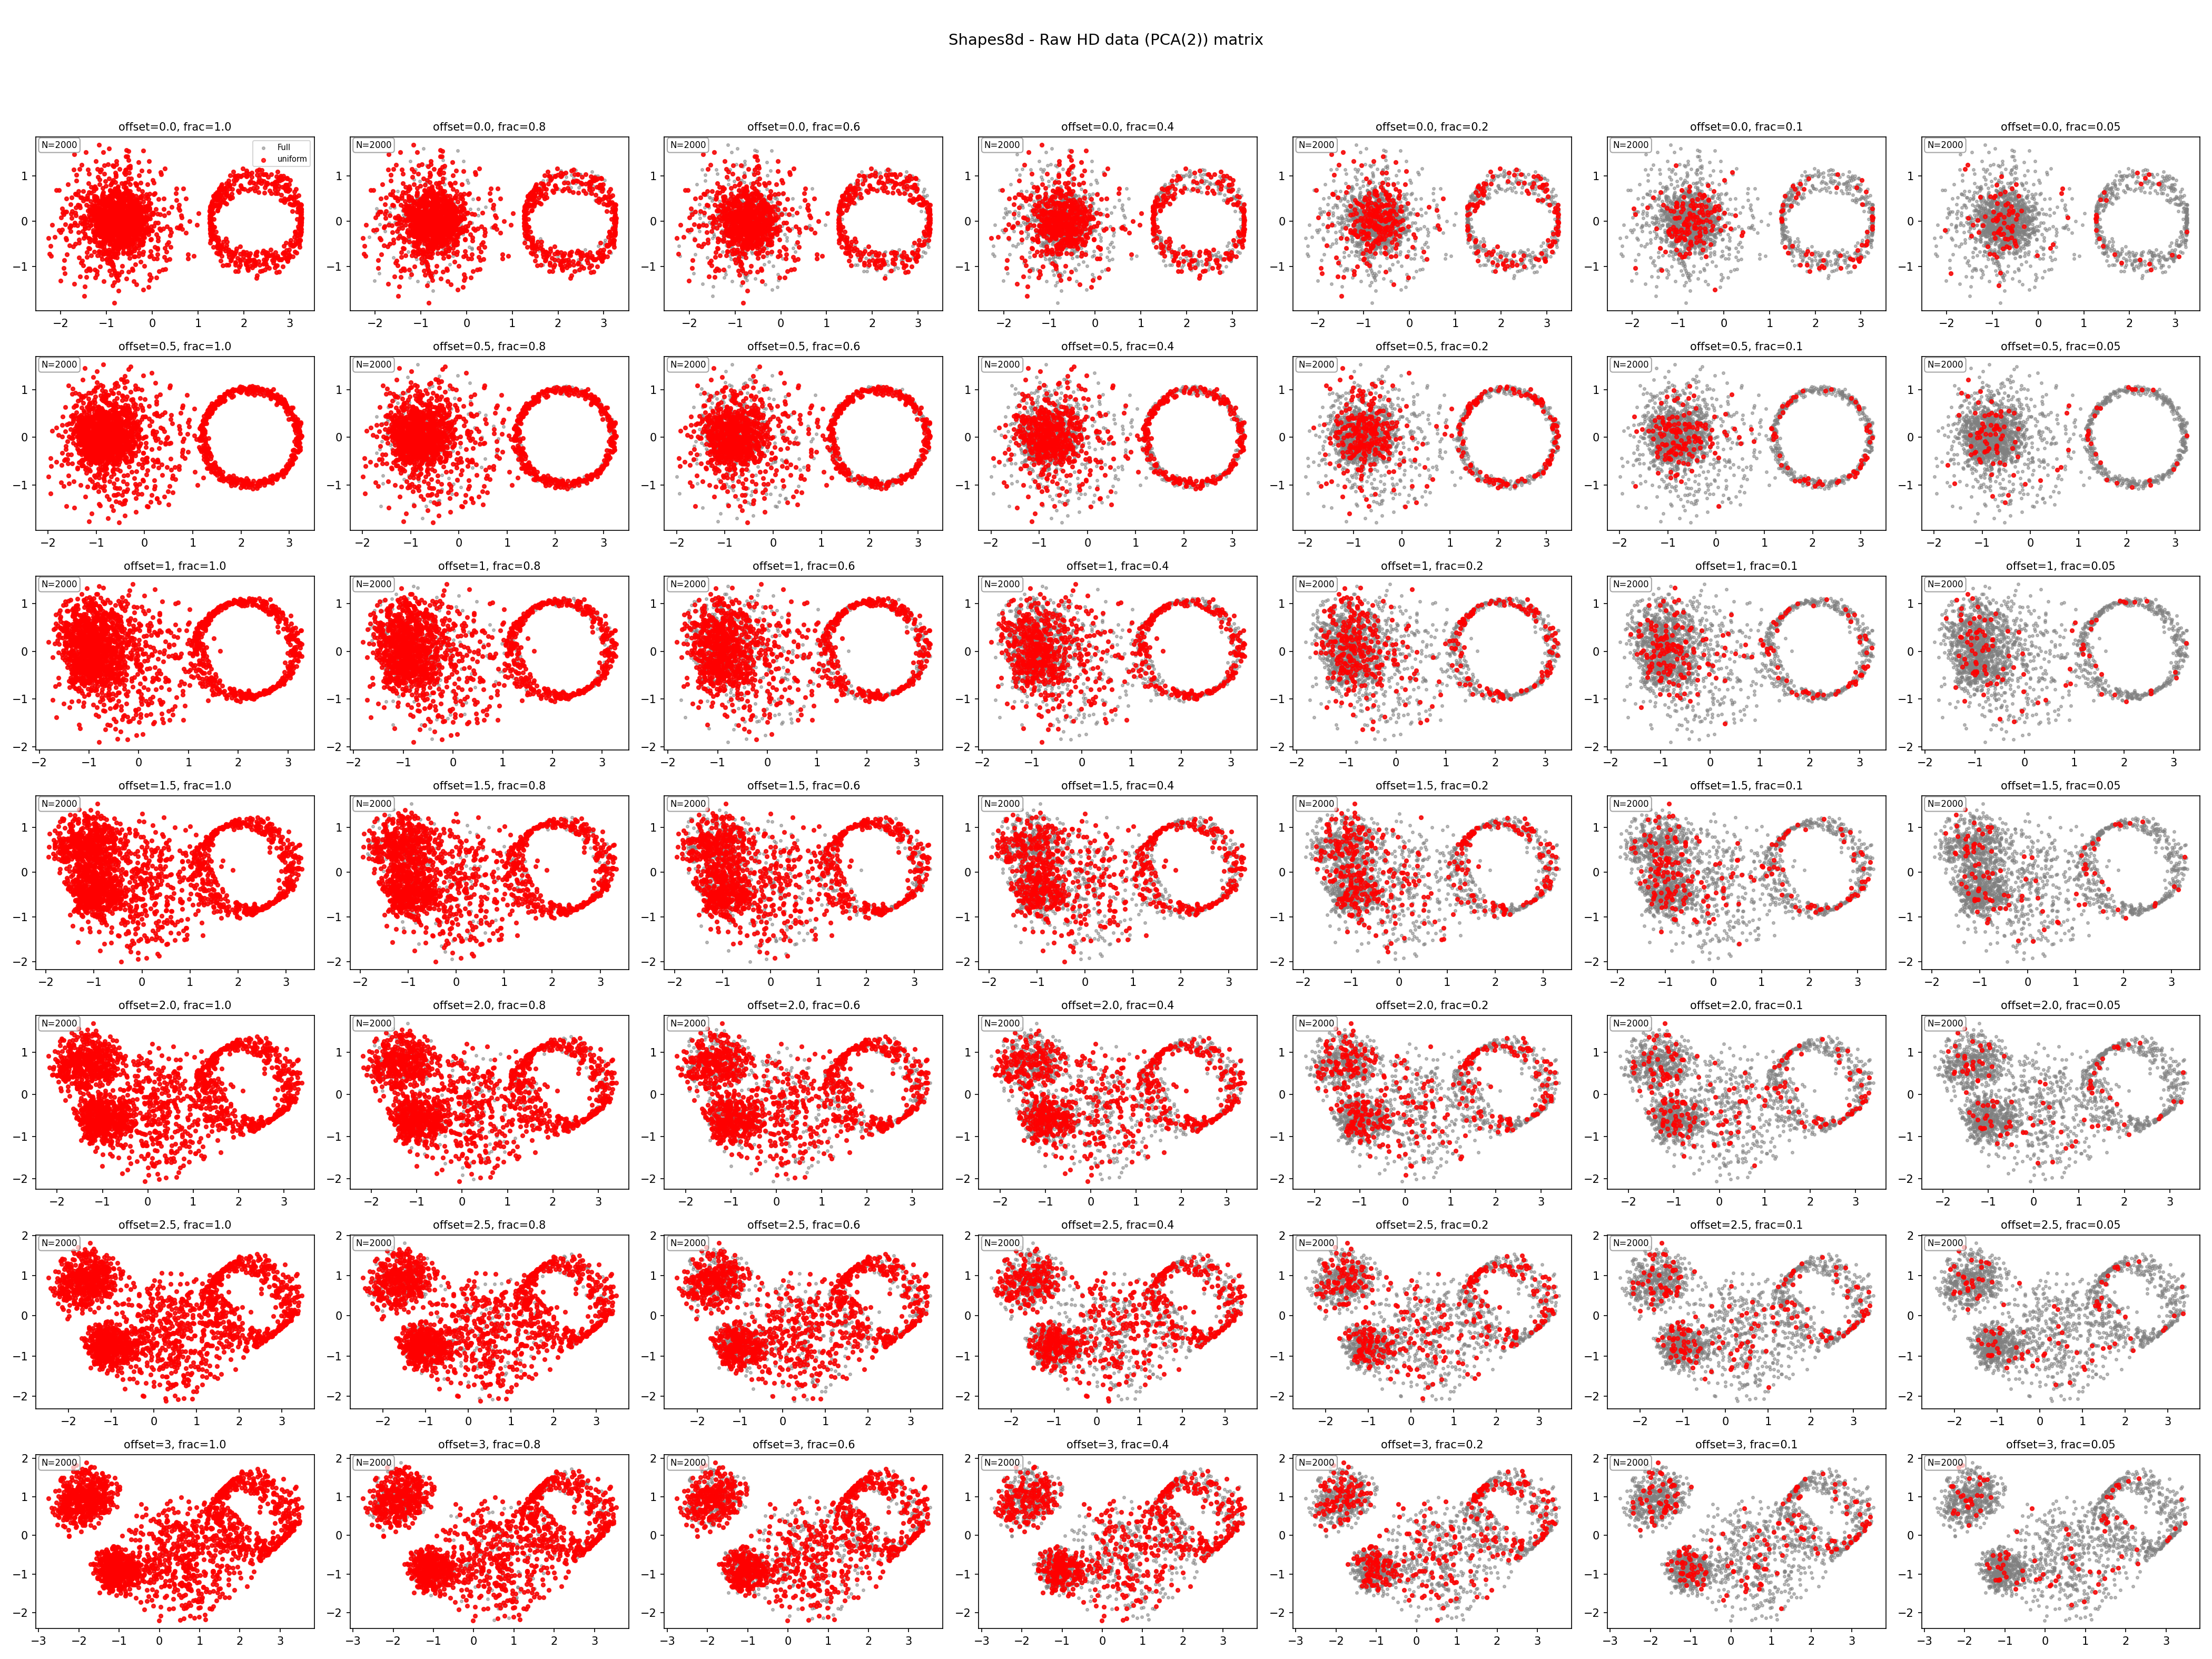
\includegraphics[trim=0pt 0pt 0pt 100pt, clip, width=0.8\linewidth]{figures/Shapes8d_matrix_hddata.png}
\caption{We generate the depicted embeddings of these objects using PCA on the first two principal components to visualize the change incurred due to varying offsets along the y axis and sampling density along the x axis. Each combination of sampling density and offset was used in the experiment.}
\label{fig:matrix-example}
\end{figure}


\subsection{Computational Considerations}
\label{app:implementation}

\paragraph{Reproducibility.}
All random seeds for sampling (both uniform and biased) are fixed for each run, ensuring that rerunning the pipeline yields identical subsets and noise realizations. Configuration parameters (offset values, sampling fractions, kernel hyperparameters) are stored in JSON files, with output appended to a single CSV file. The code used for experiments will be provided to facilitate replication and verification of results.

\paragraph{Parallelization and Optimization.}
To handle the large volume of experimental data ($\approx 100,000$ configurations), computations were parallelized using multi-processing techniques on machines with 18 cores, 5gb ram attributed to each core. Memory constraints were addressed by employing standard libraries for graph construction and manifold embedding, and using python optimal transport libraries with regularized GW functions that allowed for set relative tolerances in the precision of the solutions, thereby ensuring reasonable run-time. Further run-time optimizations via multiprocessing ensured that experiments completed within reasonable time frames without compromising the integrity of the results.


%%%%%%%%%%%%%%%%%%%%%%%%%%%%%%%%%%%%%%%%%%%%%%%%%%%%%%%%%%%%

\newpage
\section*{NeurIPS Paper Checklist}

% %%% BEGIN INSTRUCTIONS %%%
% The checklist is designed to encourage best practices for responsible machine learning research, addressing issues of reproducibility, transparency, research ethics, and societal impact. Do not remove the checklist: {\bf The papers not including the checklist will be desk rejected.} The checklist should follow the references and follow the (optional) supplemental material.  The checklist does NOT count towards the page
% limit. 

% Please read the checklist guidelines carefully for information on how to answer these questions. For each question in the checklist:
% \begin{itemize}
%     \item You should answer \answerYes{}, \answerNo{}, or \answerNA{}.
%     \item \answerNA{} means either that the question is Not Applicable for that particular paper or the relevant information is Not Available.
%     \item Please provide a short (1–2 sentence) justification right after your answer (even for NA). 
%    % \item {\bf The papers not including the checklist will be desk rejected.}
% \end{itemize}

% {\bf The checklist answers are an integral part of your paper submission.} They are visible to the reviewers, area chairs, senior area chairs, and ethics reviewers. You will be asked to also include it (after eventual revisions) with the final version of your paper, and its final version will be published with the paper.

% The reviewers of your paper will be asked to use the checklist as one of the factors in their evaluation. While "\answerYes{}" is generally preferable to "\answerNo{}", it is perfectly acceptable to answer "\answerNo{}" provided a proper justification is given (e.g., "error bars are not reported because it would be too computationally expensive" or "we were unable to find the license for the dataset we used"). In general, answering "\answerNo{}" or "\answerNA{}" is not grounds for rejection. While the questions are phrased in a binary way, we acknowledge that the true answer is often more nuanced, so please just use your best judgment and write a justification to elaborate. All supporting evidence can appear either in the main paper or the supplemental material, provided in appendix. If you answer \answerYes{} to a question, in the justification please point to the section(s) where related material for the question can be found.

% IMPORTANT, please:
% \begin{itemize}
%     \item {\bf Delete this instruction block, but keep the section heading ``NeurIPS Paper Checklist"},
%     \item  {\bf Keep the checklist subsection headings, questions/answers and guidelines below.}
%     \item {\bf Do not modify the questions and only use the provided macros for your answers}.
% \end{itemize} 
 

% %%% END INSTRUCTIONS %%%


\begin{enumerate}

\item {\bf Claims}
    \item[] Question: Do the main claims made in the abstract and introduction accurately reflect the paper's contributions and scope?
    \item[] Answer: \answerYes{} % Replace by \answerYes{}, \answerNo{}, or \answerNA{}.
    \item[] Justification: The theoretical and experimental results provide substantial evidence towards the existence of the threshold as outlined in the abstract and introduction of the paper.
    \item[] Guidelines:
    \begin{itemize}
        \item The answer NA means that the abstract and introduction do not include the claims made in the paper.
        \item The abstract and/or introduction should clearly state the claims made, including the contributions made in the paper and important assumptions and limitations. A No or NA answer to this question will not be perceived well by the reviewers. 
        \item The claims made should match theoretical and experimental results, and reflect how much the results can be expected to generalize to other settings. 
        \item It is fine to include aspirational goals as motivation as long as it is clear that these goals are not attained by the paper. 
    \end{itemize}

\item {\bf Limitations}
    \item[] Question: Does the paper discuss the limitations of the work performed by the authors?
    \item[] Answer: \answerYes{} % Replace by \answerYes{}, \answerNo{}, or \answerNA{}.
    \item[] Justification: This is included in the limitations section of the discussion, where we consider further experiments that could have been performed and other limitations.
    \item[] Guidelines:
    \begin{itemize}
        \item The answer NA means that the paper has no limitation while the answer No means that the paper has limitations, but those are not discussed in the paper. 
        \item The authors are encouraged to create a separate "Limitations" section in their paper.
        \item The paper should point out any strong assumptions and how robust the results are to violations of these assumptions (e.g., independence assumptions, noiseless settings, model well-specification, asymptotic approximations only holding locally). The authors should reflect on how these assumptions might be violated in practice and what the implications would be.
        \item The authors should reflect on the scope of the claims made, e.g., if the approach was only tested on a few datasets or with a few runs. In general, empirical results often depend on implicit assumptions, which should be articulated.
        \item The authors should reflect on the factors that influence the performance of the approach. For example, a facial recognition algorithm may perform poorly when image resolution is low or images are taken in low lighting. Or a speech-to-text system might not be used reliably to provide closed captions for online lectures because it fails to handle technical jargon.
        \item The authors should discuss the computational efficiency of the proposed algorithms and how they scale with dataset size.
        \item If applicable, the authors should discuss possible limitations of their approach to address problems of privacy and fairness.
        \item While the authors might fear that complete honesty about limitations might be used by reviewers as grounds for rejection, a worse outcome might be that reviewers discover limitations that aren't acknowledged in the paper. The authors should use their best judgment and recognize that individual actions in favor of transparency play an important role in developing norms that preserve the integrity of the community. Reviewers will be specifically instructed to not penalize honesty concerning limitations.
    \end{itemize}

\item {\bf Theory assumptions and proofs}
    \item[] Question: For each theoretical result, does the paper provide the full set of assumptions and a complete (and correct) proof?
    \item[] Answer: \answerYes{} % Replace by \answerYes{}, \answerNo{}, or \answerNA{}.
    \item[] Justification: Every theoretical result has proof sketches provided in the main text with full proofs provided in the appendix. 
    \item[] Guidelines:
    \begin{itemize}
        \item The answer NA means that the paper does not include theoretical results. 
        \item All the theorems, formulas, and proofs in the paper should be numbered and cross-referenced.
        \item All assumptions should be clearly stated or referenced in the statement of any theorems.
        \item The proofs can either appear in the main paper or the supplemental material, but if they appear in the supplemental material, the authors are encouraged to provide a short proof sketch to provide intuition. 
        \item Inversely, any informal proof provided in the core of the paper should be complemented by formal proofs provided in appendix or supplemental material.
        \item Theorems and Lemmas that the proof relies upon should be properly referenced. 
    \end{itemize}

    \item {\bf Experimental result reproducibility}
    \item[] Question: Does the paper fully disclose all the information needed to reproduce the main experimental results of the paper to the extent that it affects the main claims and/or conclusions of the paper (regardless of whether the code and data are provided or not)?
    \item[] Answer: \answerYes{} % Replace by \answerYes{}, \answerNo{}, or \answerNA{}.
    \item[] Justification: Code will be provided and made available, and all algorithmic descriptions and datasets are cited and freely available.
    \item[] Guidelines:
    \begin{itemize}
        \item The answer NA means that the paper does not include experiments.
        \item If the paper includes experiments, a No answer to this question will not be perceived well by the reviewers: Making the paper reproducible is important, regardless of whether the code and data are provided or not.
        \item If the contribution is a dataset and/or model, the authors should describe the steps taken to make their results reproducible or verifiable. 
        \item Depending on the contribution, reproducibility can be accomplished in various ways. For example, if the contribution is a novel architecture, describing the architecture fully might suffice, or if the contribution is a specific model and empirical evaluation, it may be necessary to either make it possible for others to replicate the model with the same dataset, or provide access to the model. In general. releasing code and data is often one good way to accomplish this, but reproducibility can also be provided via detailed instructions for how to replicate the results, access to a hosted model (e.g., in the case of a large language model), releasing of a model checkpoint, or other means that are appropriate to the research performed.
        \item While NeurIPS does not require releasing code, the conference does require all submissions to provide some reasonable avenue for reproducibility, which may depend on the nature of the contribution. For example
        \begin{enumerate}
            \item If the contribution is primarily a new algorithm, the paper should make it clear how to reproduce that algorithm.
            \item If the contribution is primarily a new model architecture, the paper should describe the architecture clearly and fully.
            \item If the contribution is a new model (e.g., a large language model), then there should either be a way to access this model for reproducing the results or a way to reproduce the model (e.g., with an open-source dataset or instructions for how to construct the dataset).
            \item We recognize that reproducibility may be tricky in some cases, in which case authors are welcome to describe the particular way they provide for reproducibility. In the case of closed-source models, it may be that access to the model is limited in some way (e.g., to registered users), but it should be possible for other researchers to have some path to reproducing or verifying the results.
        \end{enumerate}
    \end{itemize}


\item {\bf Open access to data and code}
    \item[] Question: Does the paper provide open access to the data and code, with sufficient instructions to faithfully reproduce the main experimental results, as described in supplemental material?
    \item[] Answer: \answerYes{} % Replace by \answerYes{}, \answerNo{}, or \answerNA{}.
    \item[] Justification: Code to reproduce the synthetic and real data results will be provided. The data used is already freely available.
    \item[] Guidelines:
    \begin{itemize}
        \item The answer NA means that paper does not include experiments requiring code.
        \item Please see the NeurIPS code and data submission guidelines (\url{https://nips.cc/public/guides/CodeSubmissionPolicy}) for more details.
        \item While we encourage the release of code and data, we understand that this might not be possible, so “No” is an acceptable answer. Papers cannot be rejected simply for not including code, unless this is central to the contribution (e.g., for a new open-source benchmark).
        \item The instructions should contain the exact command and environment needed to run to reproduce the results. See the NeurIPS code and data submission guidelines (\url{https://nips.cc/public/guides/CodeSubmissionPolicy}) for more details.
        \item The authors should provide instructions on data access and preparation, including how to access the raw data, preprocessed data, intermediate data, and generated data, etc.
        \item The authors should provide scripts to reproduce all experimental results for the new proposed method and baselines. If only a subset of experiments are reproducible, they should state which ones are omitted from the script and why.
        \item At submission time, to preserve anonymity, the authors should release anonymized versions (if applicable).
        \item Providing as much information as possible in supplemental material (appended to the paper) is recommended, but including URLs to data and code is permitted.
    \end{itemize}


\item {\bf Experimental setting/details}
    \item[] Question: Does the paper specify all the training and test details (e.g., data splits, hyperparameters, how they were chosen, type of optimizer, etc.) necessary to understand the results?
    \item[] Answer: \answerYes{} % Replace by \answerYes{}, \answerNo{}, or \answerNA{}.
    \item[] Justification: This information is provided in the appendix.
    \item[] Guidelines:
    \begin{itemize}
        \item The answer NA means that the paper does not include experiments.
        \item The experimental setting should be presented in the core of the paper to a level of detail that is necessary to appreciate the results and make sense of them.
        \item The full details can be provided either with the code, in appendix, or as supplemental material.
    \end{itemize}

\item {\bf Experiment statistical significance}
    \item[] Question: Does the paper report error bars suitably and correctly defined or other appropriate information about the statistical significance of the experiments?
    \item[] Answer: \answerYes{} % Replace by \answerYes{}, \answerNo{}, or \answerNA{}.
    \item[] Justification: Error bars are included on figures where possible and relevant in the empirical results section of the paper.
    \item[] Guidelines:
    \begin{itemize}
        \item The answer NA means that the paper does not include experiments.
        \item The authors should answer "Yes" if the results are accompanied by error bars, confidence intervals, or statistical significance tests, at least for the experiments that support the main claims of the paper.
        \item The factors of variability that the error bars are capturing should be clearly stated (for example, train/test split, initialization, random drawing of some parameter, or overall run with given experimental conditions).
        \item The method for calculating the error bars should be explained (closed form formula, call to a library function, bootstrap, etc.)
        \item The assumptions made should be given (e.g., Normally distributed errors).
        \item It should be clear whether the error bar is the standard deviation or the standard error of the mean.
        \item It is OK to report 1-sigma error bars, but one should state it. The authors should preferably report a 2-sigma error bar than state that they have a 96\% CI, if the hypothesis of Normality of errors is not verified.
        \item For asymmetric distributions, the authors should be careful not to show in tables or figures symmetric error bars that would yield results that are out of range (e.g. negative error rates).
        \item If error bars are reported in tables or plots, The authors should explain in the text how they were calculated and reference the corresponding figures or tables in the text.
    \end{itemize}

\item {\bf Experiments compute resources}
    \item[] Question: For each experiment, does the paper provide sufficient information on the computer resources (type of compute workers, memory, time of execution) needed to reproduce the experiments?
    \item[] Answer: \answerYes{} % Replace by \answerYes{}, \answerNo{}, or \answerNA{}.
    \item[] Justification: The relevant information for resources is provided in the appendix.
    \item[] Guidelines:
    \begin{itemize}
        \item The answer NA means that the paper does not include experiments.
        \item The paper should indicate the type of compute workers CPU or GPU, internal cluster, or cloud provider, including relevant memory and storage.
        \item The paper should provide the amount of compute required for each of the individual experimental runs as well as estimate the total compute. 
        \item The paper should disclose whether the full research project required more compute than the experiments reported in the paper (e.g., preliminary or failed experiments that didn't make it into the paper). 
    \end{itemize}
    
\item {\bf Code of ethics}
    \item[] Question: Does the research conducted in the paper conform, in every respect, with the NeurIPS Code of Ethics \url{https://neurips.cc/public/EthicsGuidelines}?
    \item[] Answer: \answerYes{} % Replace by \answerYes{}, \answerNo{}, or \answerNA{}.
    \item[] Justification: The research conforms to the code of ethics.
    \item[] Guidelines:
    \begin{itemize}
        \item The answer NA means that the authors have not reviewed the NeurIPS Code of Ethics.
        \item If the authors answer No, they should explain the special circumstances that require a deviation from the Code of Ethics.
        \item The authors should make sure to preserve anonymity (e.g., if there is a special consideration due to laws or regulations in their jurisdiction).
    \end{itemize}


\item {\bf Broader impacts}
    \item[] Question: Does the paper discuss both potential positive societal impacts and negative societal impacts of the work performed?
    \item[] Answer: \answerYes{} % Replace by \answerYes{}, \answerNo{}, or \answerNA{}.
    \item[] Justification: We touch upon this in the conclusion of the paper.
    \item[] Guidelines:
    \begin{itemize}
        \item The answer NA means that there is no societal impact of the work performed.
        \item If the authors answer NA or No, they should explain why their work has no societal impact or why the paper does not address societal impact.
        \item Examples of negative societal impacts include potential malicious or unintended uses (e.g., disinformation, generating fake profiles, surveillance), fairness considerations (e.g., deployment of technologies that could make decisions that unfairly impact specific groups), privacy considerations, and security considerations.
        \item The conference expects that many papers will be foundational research and not tied to particular applications, let alone deployments. However, if there is a direct path to any negative applications, the authors should point it out. For example, it is legitimate to point out that an improvement in the quality of generative models could be used to generate deepfakes for disinformation. On the other hand, it is not needed to point out that a generic algorithm for optimizing neural networks could enable people to train models that generate Deepfakes faster.
        \item The authors should consider possible harms that could arise when the technology is being used as intended and functioning correctly, harms that could arise when the technology is being used as intended but gives incorrect results, and harms following from (intentional or unintentional) misuse of the technology.
        \item If there are negative societal impacts, the authors could also discuss possible mitigation strategies (e.g., gated release of models, providing defenses in addition to attacks, mechanisms for monitoring misuse, mechanisms to monitor how a system learns from feedback over time, improving the efficiency and accessibility of ML).
    \end{itemize}
    
\item {\bf Safeguards}
    \item[] Question: Does the paper describe safeguards that have been put in place for responsible release of data or models that have a high risk for misuse (e.g., pretrained language models, image generators, or scraped datasets)?
    \item[] Answer: \answerNA{} % Replace by \answerYes{}, \answerNo{}, or \answerNA{}.
    \item[] Justification: The provided results pose no such risk for misuse in the manner outlined above.
    \item[] Guidelines:
    \begin{itemize}
        \item The answer NA means that the paper poses no such risks.
        \item Released models that have a high risk for misuse or dual-use should be released with necessary safeguards to allow for controlled use of the model, for example by requiring that users adhere to usage guidelines or restrictions to access the model or implementing safety filters. 
        \item Datasets that have been scraped from the Internet could pose safety risks. The authors should describe how they avoided releasing unsafe images.
        \item We recognize that providing effective safeguards is challenging, and many papers do not require this, but we encourage authors to take this into account and make a best faith effort.
    \end{itemize}

\item {\bf Licenses for existing assets}
    \item[] Question: Are the creators or original owners of assets (e.g., code, data, models), used in the paper, properly credited and are the license and terms of use explicitly mentioned and properly respected?
    \item[] Answer: \answerYes{} % Replace by \answerYes{}, \answerNo{}, or \answerNA{}.
    \item[] Justification: All the data and code utilized for empirical testing were explicitly mentioned and cited appropriately.
    \item[] Guidelines:
    \begin{itemize}
        \item The answer NA means that the paper does not use existing assets.
        \item The authors should cite the original paper that produced the code package or dataset.
        \item The authors should state which version of the asset is used and, if possible, include a URL.
        \item The name of the license (e.g., CC-BY 4.0) should be included for each asset.
        \item For scraped data from a particular source (e.g., website), the copyright and terms of service of that source should be provided.
        \item If assets are released, the license, copyright information, and terms of use in the package should be provided. For popular datasets, \url{paperswithcode.com/datasets} has curated licenses for some datasets. Their licensing guide can help determine the license of a dataset.
        \item For existing datasets that are re-packaged, both the original license and the license of the derived asset (if it has changed) should be provided.
        \item If this information is not available online, the authors are encouraged to reach out to the asset's creators.
    \end{itemize}

\item {\bf New assets}
    \item[] Question: Are new assets introduced in the paper well documented and is the documentation provided alongside the assets?
    \item[] Answer: \answerYes{} % Replace by \answerYes{}, \answerNo{}, or \answerNA{}.
    \item[] Justification: All documentation involving data used for empirical experiments where provided.
    \item[] Guidelines:
    \begin{itemize}
        \item The answer NA means that the paper does not release new assets.
        \item Researchers should communicate the details of the dataset/code/model as part of their submissions via structured templates. This includes details about training, license, limitations, etc. 
        \item The paper should discuss whether and how consent was obtained from people whose asset is used.
        \item At submission time, remember to anonymize your assets (if applicable). You can either create an anonymized URL or include an anonymized zip file.
    \end{itemize}

\item {\bf Crowdsourcing and research with human subjects}
    \item[] Question: For crowdsourcing experiments and research with human subjects, does the paper include the full text of instructions given to participants and screenshots, if applicable, as well as details about compensation (if any)? 
    \item[] Answer: \answerNA{} % Replace by \answerYes{}, \answerNo{}, or \answerNA{}.
    \item[] Justification: No crowdsourcing or human subject research were involved in this work.
    \item[] Guidelines:
    \begin{itemize}
        \item The answer NA means that the paper does not involve crowdsourcing nor research with human subjects.
        \item Including this information in the supplemental material is fine, but if the main contribution of the paper involves human subjects, then as much detail as possible should be included in the main paper. 
        \item According to the NeurIPS Code of Ethics, workers involved in data collection, curation, or other labor should be paid at least the minimum wage in the country of the data collector. 
    \end{itemize}

\item {\bf Institutional review board (IRB) approvals or equivalent for research with human subjects}
    \item[] Question: Does the paper describe potential risks incurred by study participants, whether such risks were disclosed to the subjects, and whether Institutional Review Board (IRB) approvals (or an equivalent approval/review based on the requirements of your country or institution) were obtained?
    \item[] Answer: \answerNA{} % Replace by \answerYes{}, \answerNo{}, or \answerNA{}.
    \item[] Justification: No IRB approvals or equivalent practices were relevant for this work.
    \item[] Guidelines:
    \begin{itemize}
        \item The answer NA means that the paper does not involve crowdsourcing nor research with human subjects.
        \item Depending on the country in which research is conducted, IRB approval (or equivalent) may be required for any human subjects research. If you obtained IRB approval, you should clearly state this in the paper. 
        \item We recognize that the procedures for this may vary significantly between institutions and locations, and we expect authors to adhere to the NeurIPS Code of Ethics and the guidelines for their institution. 
        \item For initial submissions, do not include any information that would break anonymity (if applicable), such as the institution conducting the review.
    \end{itemize}

\item {\bf Declaration of LLM usage}
    \item[] Question: Does the paper describe the usage of LLMs if it is an important, original, or non-standard component of the core methods in this research? Note that if the LLM is used only for writing, editing, or formatting purposes and does not impact the core methodology, scientific rigorousness, or originality of the research, declaration is not required.
    %this research? 
    \item[] Answer: \answerNA{} % Replace by \answerYes{}, \answerNo{}, or \answerNA{}.
    \item[] Justification: As stated in the question, the core method does not involve LLMs and is thus not applicable.
    \item[] Guidelines:
    \begin{itemize}
        \item The answer NA means that the core method development in this research does not involve LLMs as any important, original, or non-standard components.
        \item Please refer to our LLM policy (\url{https://neurips.cc/Conferences/2025/LLM}) for what should or should not be described.
    \end{itemize}

\end{enumerate}


\end{document}

